\documentclass{book}
\usepackage[a4paper,top=2.5cm,bottom=2.5cm,left=2.5cm,right=2.5cm]{geometry}
\usepackage{makeidx}
\usepackage{natbib}
\usepackage{graphicx}
\usepackage{multicol}
\usepackage{float}
\usepackage{listings}
\usepackage{color}
\usepackage{ifthen}
\usepackage[table]{xcolor}
\usepackage{textcomp}
\usepackage{alltt}
\usepackage{ifpdf}
\ifpdf
\usepackage[pdftex,
            pagebackref=true,
            colorlinks=true,
            linkcolor=blue,
            unicode
           ]{hyperref}
\else
\usepackage[ps2pdf,
            pagebackref=true,
            colorlinks=true,
            linkcolor=blue,
            unicode
           ]{hyperref}
\usepackage{pspicture}
\fi
\usepackage[utf8]{inputenc}
\usepackage{mathptmx}
\usepackage[scaled=.90]{helvet}
\usepackage{courier}
\usepackage{sectsty}
\usepackage{amssymb}
\usepackage[titles]{tocloft}
\usepackage{doxygen}
\lstset{language=C++,inputencoding=utf8,basicstyle=\footnotesize,breaklines=true,breakatwhitespace=true,tabsize=8,numbers=left }
\makeindex
\setcounter{tocdepth}{3}
\renewcommand{\footrulewidth}{0.4pt}
\renewcommand{\familydefault}{\sfdefault}
\hfuzz=15pt
\setlength{\emergencystretch}{15pt}
\hbadness=750
\tolerance=750
\begin{document}
\hypersetup{pageanchor=false,citecolor=blue}
\begin{titlepage}
\vspace*{7cm}
\begin{center}
{\Large Network-\/\-Music \\[1ex]\large 0.\-1 }\\
\vspace*{1cm}
{\large Generated by Doxygen 1.8.1.2}\\
\vspace*{0.5cm}
{\small Wed Apr 29 2015 17:40:05}\\
\end{center}
\end{titlepage}
\clearemptydoublepage
\pagenumbering{roman}
\tableofcontents
\clearemptydoublepage
\pagenumbering{arabic}
\hypersetup{pageanchor=true,citecolor=blue}
\chapter{Network-\/\-Music}
\label{md_README}
\hypertarget{md_README}{}
\input{md__r_e_a_d_m_e}
\chapter{Namespace Index}
\section{Namespace List}
Here is a list of all namespaces with brief descriptions\-:\begin{DoxyCompactList}
\item\contentsline{section}{\hyperlink{namespacepacketprocess}{packetprocess} }{\pageref{namespacepacketprocess}}{}
\end{DoxyCompactList}

\chapter{Class Index}
\section{Class List}
Here are the classes, structs, unions and interfaces with brief descriptions\-:\begin{DoxyCompactList}
\item\contentsline{section}{\hyperlink{class_audio_graph}{Audio\-Graph} }{\pageref{class_audio_graph}}{}
\item\contentsline{section}{\hyperlink{class_audio_test}{Audio\-Test} }{\pageref{class_audio_test}}{}
\item\contentsline{section}{\hyperlink{class_generator}{Generator} }{\pageref{class_generator}}{}
\item\contentsline{section}{\hyperlink{class_main_window}{Main\-Window} }{\pageref{class_main_window}}{}
\item\contentsline{section}{\hyperlink{class_packet_capturer}{Packet\-Capturer} }{\pageref{class_packet_capturer}}{}
\item\contentsline{section}{\hyperlink{structpacketprocess_1_1sniff__ethernet}{packetprocess\-::sniff\-\_\-ethernet} }{\pageref{structpacketprocess_1_1sniff__ethernet}}{}
\item\contentsline{section}{\hyperlink{structpacketprocess_1_1sniff__ip}{packetprocess\-::sniff\-\_\-ip} }{\pageref{structpacketprocess_1_1sniff__ip}}{}
\item\contentsline{section}{\hyperlink{structpacketprocess_1_1sniff__tcp}{packetprocess\-::sniff\-\_\-tcp} }{\pageref{structpacketprocess_1_1sniff__tcp}}{}
\item\contentsline{section}{\hyperlink{classtone}{tone} }{\pageref{classtone}}{}
\item\contentsline{section}{\hyperlink{class_tone_manager}{Tone\-Manager} }{\pageref{class_tone_manager}}{}
\item\contentsline{section}{\hyperlink{struct_tone_object}{Tone\-Object} }{\pageref{struct_tone_object}}{}
\end{DoxyCompactList}

\chapter{File Index}
\section{File List}
Here is a list of all files with brief descriptions\-:\begin{DoxyCompactList}
\item\contentsline{section}{Network-\/\-Music/\hyperlink{audiograph_8cpp}{audiograph.\-cpp} }{\pageref{audiograph_8cpp}}{}
\item\contentsline{section}{Network-\/\-Music/\hyperlink{audiograph_8h}{audiograph.\-h} }{\pageref{audiograph_8h}}{}
\item\contentsline{section}{Network-\/\-Music/\hyperlink{audiooutput_8cpp}{audiooutput.\-cpp} }{\pageref{audiooutput_8cpp}}{}
\item\contentsline{section}{Network-\/\-Music/\hyperlink{audiooutput_8h}{audiooutput.\-h} }{\pageref{audiooutput_8h}}{}
\item\contentsline{section}{Network-\/\-Music/\hyperlink{generator_8cpp}{generator.\-cpp} }{\pageref{generator_8cpp}}{}
\item\contentsline{section}{Network-\/\-Music/\hyperlink{generator_8h}{generator.\-h} }{\pageref{generator_8h}}{}
\item\contentsline{section}{Network-\/\-Music/\hyperlink{main_8cpp}{main.\-cpp} }{\pageref{main_8cpp}}{}
\item\contentsline{section}{Network-\/\-Music/\hyperlink{mainwindow_8cpp}{mainwindow.\-cpp} }{\pageref{mainwindow_8cpp}}{}
\item\contentsline{section}{Network-\/\-Music/\hyperlink{mainwindow_8h}{mainwindow.\-h} }{\pageref{mainwindow_8h}}{}
\item\contentsline{section}{Network-\/\-Music/\hyperlink{packetcapturer_8cpp}{packetcapturer.\-cpp} }{\pageref{packetcapturer_8cpp}}{}
\item\contentsline{section}{Network-\/\-Music/\hyperlink{packetcapturer_8h}{packetcapturer.\-h} }{\pageref{packetcapturer_8h}}{}
\item\contentsline{section}{Network-\/\-Music/\hyperlink{tone_8cpp}{tone.\-cpp} }{\pageref{tone_8cpp}}{}
\item\contentsline{section}{Network-\/\-Music/\hyperlink{tone_8h}{tone.\-h} }{\pageref{tone_8h}}{}
\item\contentsline{section}{Network-\/\-Music/\hyperlink{tonemanager_8cpp}{tonemanager.\-cpp} }{\pageref{tonemanager_8cpp}}{}
\item\contentsline{section}{Network-\/\-Music/\hyperlink{tonemanager_8h}{tonemanager.\-h} }{\pageref{tonemanager_8h}}{}
\end{DoxyCompactList}

\chapter{Namespace Documentation}
\hypertarget{namespacepacketprocess}{\section{packetprocess Namespace Reference}
\label{namespacepacketprocess}\index{packetprocess@{packetprocess}}
}
\subsection*{Classes}
\begin{DoxyCompactItemize}
\item 
struct \hyperlink{structpacketprocess_1_1sniff__ethernet}{sniff\-\_\-ethernet}
\item 
struct \hyperlink{structpacketprocess_1_1sniff__ip}{sniff\-\_\-ip}
\item 
struct \hyperlink{structpacketprocess_1_1sniff__tcp}{sniff\-\_\-tcp}
\end{DoxyCompactItemize}
\subsection*{Typedefs}
\begin{DoxyCompactItemize}
\item 
typedef u\-\_\-int \hyperlink{namespacepacketprocess_a18e81a7f74513cbc9f8881ee72f67abe}{tcp\-\_\-seq}
\end{DoxyCompactItemize}
\subsection*{Functions}
\begin{DoxyCompactItemize}
\item 
void \hyperlink{namespacepacketprocess_a17240af943c2d732bb5242e802445a5f}{Callback\-\_\-\-Process\-Packet} (u\-\_\-char $\ast$useless, const pcap\-\_\-pkthdr $\ast$pkthdr, const u\-\_\-char $\ast$packet)
\end{DoxyCompactItemize}
\subsection*{Variables}
\begin{DoxyCompactItemize}
\item 
u\-\_\-short \hyperlink{namespacepacketprocess_a0ffda1e178a79656e927189b103e8708}{recent\-Freq} = 100
\item 
Q\-Object $\ast$ \hyperlink{namespacepacketprocess_ad98eea621960299d54ed1535bf3a605e}{parent}
\end{DoxyCompactItemize}


\subsection{Typedef Documentation}
\hypertarget{namespacepacketprocess_a18e81a7f74513cbc9f8881ee72f67abe}{\index{packetprocess@{packetprocess}!tcp\-\_\-seq@{tcp\-\_\-seq}}
\index{tcp\-\_\-seq@{tcp\-\_\-seq}!packetprocess@{packetprocess}}
\subsubsection[{tcp\-\_\-seq}]{\setlength{\rightskip}{0pt plus 5cm}typedef u\-\_\-int {\bf packetprocess\-::tcp\-\_\-seq}}}\label{namespacepacketprocess_a18e81a7f74513cbc9f8881ee72f67abe}


\subsection{Function Documentation}
\hypertarget{namespacepacketprocess_a17240af943c2d732bb5242e802445a5f}{\index{packetprocess@{packetprocess}!Callback\-\_\-\-Process\-Packet@{Callback\-\_\-\-Process\-Packet}}
\index{Callback\-\_\-\-Process\-Packet@{Callback\-\_\-\-Process\-Packet}!packetprocess@{packetprocess}}
\subsubsection[{Callback\-\_\-\-Process\-Packet}]{\setlength{\rightskip}{0pt plus 5cm}void packetprocess\-::\-Callback\-\_\-\-Process\-Packet (
\begin{DoxyParamCaption}
\item[{u\-\_\-char $\ast$}]{useless, }
\item[{const pcap\-\_\-pkthdr $\ast$}]{pkthdr, }
\item[{const u\-\_\-char $\ast$}]{packet}
\end{DoxyParamCaption}
)}}\label{namespacepacketprocess_a17240af943c2d732bb5242e802445a5f}


Here is the call graph for this function\-:
\nopagebreak
\begin{figure}[H]
\begin{center}
\leavevmode
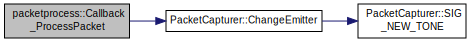
\includegraphics[width=350pt]{namespacepacketprocess_a17240af943c2d732bb5242e802445a5f_cgraph}
\end{center}
\end{figure}




Here is the caller graph for this function\-:\nopagebreak
\begin{figure}[H]
\begin{center}
\leavevmode
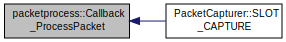
\includegraphics[width=350pt]{namespacepacketprocess_a17240af943c2d732bb5242e802445a5f_icgraph}
\end{center}
\end{figure}




\subsection{Variable Documentation}
\hypertarget{namespacepacketprocess_ad98eea621960299d54ed1535bf3a605e}{\index{packetprocess@{packetprocess}!parent@{parent}}
\index{parent@{parent}!packetprocess@{packetprocess}}
\subsubsection[{parent}]{\setlength{\rightskip}{0pt plus 5cm}Q\-Object$\ast$ packetprocess\-::parent}}\label{namespacepacketprocess_ad98eea621960299d54ed1535bf3a605e}
\hypertarget{namespacepacketprocess_a0ffda1e178a79656e927189b103e8708}{\index{packetprocess@{packetprocess}!recent\-Freq@{recent\-Freq}}
\index{recent\-Freq@{recent\-Freq}!packetprocess@{packetprocess}}
\subsubsection[{recent\-Freq}]{\setlength{\rightskip}{0pt plus 5cm}u\-\_\-short packetprocess\-::recent\-Freq = 100}}\label{namespacepacketprocess_a0ffda1e178a79656e927189b103e8708}

\chapter{Class Documentation}
\hypertarget{class_audio_graph}{\section{Audio\-Graph Class Reference}
\label{class_audio_graph}\index{Audio\-Graph@{Audio\-Graph}}
}


{\ttfamily \#include $<$audiograph.\-h$>$}

\subsection*{Public Member Functions}
\begin{DoxyCompactItemize}
\item 
\hyperlink{class_audio_graph_a24421353ce7ac296ffe9df744c91b491}{Audio\-Graph} (Q3\-D\-Scatter $\ast$scatter=0)
\item 
void \hyperlink{class_audio_graph_a317bd8becbb2be554a2a3c8b03c35e1c}{Add\-Data} (int value)
\end{DoxyCompactItemize}
\subsection*{Public Attributes}
\begin{DoxyCompactItemize}
\item 
Q\-Widget $\ast$ \hyperlink{class_audio_graph_a1a29a297d2fd010222069f42b978e883}{container}
\item 
Q3\-D\-Scatter $\ast$ \hyperlink{class_audio_graph_a547436a673bb2e1772148b4769c223f6}{m\-\_\-graph}
\end{DoxyCompactItemize}
\subsection*{Protected Attributes}
\begin{DoxyCompactItemize}
\item 
float \hyperlink{class_audio_graph_a99a167dc71ac6a34f248577836a4a5ce}{time}
\item 
Q\-Timer $\ast$ \hyperlink{class_audio_graph_a197d420df22017259456303e0d702a55}{timer}
\end{DoxyCompactItemize}


\subsection{Constructor \& Destructor Documentation}
\hypertarget{class_audio_graph_a24421353ce7ac296ffe9df744c91b491}{\index{Audio\-Graph@{Audio\-Graph}!Audio\-Graph@{Audio\-Graph}}
\index{Audio\-Graph@{Audio\-Graph}!AudioGraph@{Audio\-Graph}}
\subsubsection[{Audio\-Graph}]{\setlength{\rightskip}{0pt plus 5cm}Audio\-Graph\-::\-Audio\-Graph (
\begin{DoxyParamCaption}
\item[{Q3\-D\-Scatter $\ast$}]{scatter = {\ttfamily 0}}
\end{DoxyParamCaption}
)\hspace{0.3cm}{\ttfamily [explicit]}}}\label{class_audio_graph_a24421353ce7ac296ffe9df744c91b491}


\subsection{Member Function Documentation}
\hypertarget{class_audio_graph_a317bd8becbb2be554a2a3c8b03c35e1c}{\index{Audio\-Graph@{Audio\-Graph}!Add\-Data@{Add\-Data}}
\index{Add\-Data@{Add\-Data}!AudioGraph@{Audio\-Graph}}
\subsubsection[{Add\-Data}]{\setlength{\rightskip}{0pt plus 5cm}void Audio\-Graph\-::\-Add\-Data (
\begin{DoxyParamCaption}
\item[{int}]{value}
\end{DoxyParamCaption}
)}}\label{class_audio_graph_a317bd8becbb2be554a2a3c8b03c35e1c}


\subsection{Member Data Documentation}
\hypertarget{class_audio_graph_a1a29a297d2fd010222069f42b978e883}{\index{Audio\-Graph@{Audio\-Graph}!container@{container}}
\index{container@{container}!AudioGraph@{Audio\-Graph}}
\subsubsection[{container}]{\setlength{\rightskip}{0pt plus 5cm}Q\-Widget$\ast$ Audio\-Graph\-::container}}\label{class_audio_graph_a1a29a297d2fd010222069f42b978e883}
\hypertarget{class_audio_graph_a547436a673bb2e1772148b4769c223f6}{\index{Audio\-Graph@{Audio\-Graph}!m\-\_\-graph@{m\-\_\-graph}}
\index{m\-\_\-graph@{m\-\_\-graph}!AudioGraph@{Audio\-Graph}}
\subsubsection[{m\-\_\-graph}]{\setlength{\rightskip}{0pt plus 5cm}Q3\-D\-Scatter$\ast$ Audio\-Graph\-::m\-\_\-graph}}\label{class_audio_graph_a547436a673bb2e1772148b4769c223f6}
\hypertarget{class_audio_graph_a99a167dc71ac6a34f248577836a4a5ce}{\index{Audio\-Graph@{Audio\-Graph}!time@{time}}
\index{time@{time}!AudioGraph@{Audio\-Graph}}
\subsubsection[{time}]{\setlength{\rightskip}{0pt plus 5cm}float Audio\-Graph\-::time\hspace{0.3cm}{\ttfamily [protected]}}}\label{class_audio_graph_a99a167dc71ac6a34f248577836a4a5ce}
\hypertarget{class_audio_graph_a197d420df22017259456303e0d702a55}{\index{Audio\-Graph@{Audio\-Graph}!timer@{timer}}
\index{timer@{timer}!AudioGraph@{Audio\-Graph}}
\subsubsection[{timer}]{\setlength{\rightskip}{0pt plus 5cm}Q\-Timer$\ast$ Audio\-Graph\-::timer\hspace{0.3cm}{\ttfamily [protected]}}}\label{class_audio_graph_a197d420df22017259456303e0d702a55}


The documentation for this class was generated from the following files\-:\begin{DoxyCompactItemize}
\item 
Network-\/\-Music/\hyperlink{audiograph_8h}{audiograph.\-h}\item 
Network-\/\-Music/\hyperlink{audiograph_8cpp}{audiograph.\-cpp}\end{DoxyCompactItemize}

\hypertarget{class_audio_test}{\section{Audio\-Test Class Reference}
\label{class_audio_test}\index{Audio\-Test@{Audio\-Test}}
}


{\ttfamily \#include $<$audiooutput.\-h$>$}



Collaboration diagram for Audio\-Test\-:
\nopagebreak
\begin{figure}[H]
\begin{center}
\leavevmode
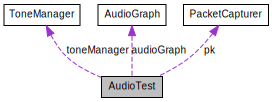
\includegraphics[width=344pt]{class_audio_test__coll__graph}
\end{center}
\end{figure}
\subsection*{Signals}
\begin{DoxyCompactItemize}
\item 
void \hyperlink{class_audio_test_a97c30aeee89c952e4f9e213d26883da6}{Volume\-Changed} (int)
\item 
void \hyperlink{class_audio_test_a44db884ba0eaf1838099d0aeb29a04d6}{S\-I\-G\-N\-A\-L\-\_\-\-B\-E\-G\-I\-N\-\_\-\-T\-O\-N\-E\-S} ()
\item 
void \hyperlink{class_audio_test_a7f324e3db9ffe815a1c1b3af12e520a5}{S\-I\-G\-N\-A\-L\-\_\-\-B\-E\-G\-I\-N\-\_\-\-C\-A\-P\-T\-U\-R\-E} ()
\end{DoxyCompactItemize}
\subsection*{Public Member Functions}
\begin{DoxyCompactItemize}
\item 
\hyperlink{class_audio_test_a086084868d3cadb9b4c8e1a8549425e9}{Audio\-Test} ()
\item 
void \hyperlink{class_audio_test_a717dfe69311252d9890838a250946064}{Setup} ()
\end{DoxyCompactItemize}
\subsection*{Protected Member Functions}
\begin{DoxyCompactItemize}
\item 
void \hyperlink{class_audio_test_a1b80cfb92faf38273d77a908ad1ef803}{initialize\-Window} ()
\item 
void \hyperlink{class_audio_test_a80b6f4ce52947f96d9f243cf93d04a46}{initialize\-Audio} ()
\item 
void \hyperlink{class_audio_test_a9a38ae87dce3988e4560832475be32ca}{create\-Audio\-Output} ()
\end{DoxyCompactItemize}
\subsection*{Protected Attributes}
\begin{DoxyCompactItemize}
\item 
Q\-Combo\-Box $\ast$ \hyperlink{class_audio_test_a9da9104fab5169ae9016993136b22e2e}{m\-\_\-network\-Device\-Box}
\item 
Q\-Label $\ast$ \hyperlink{class_audio_test_a7cc252683f93e389b0783a8b34671665}{m\-\_\-volume\-Label}
\item 
Q\-Slider $\ast$ \hyperlink{class_audio_test_a822b1b9f3ac4cd529e90187f713a0eb8}{m\-\_\-volume\-Slider}
\item 
Q\-Slider $\ast$ \hyperlink{class_audio_test_ab5999227ac75e0ecd7012e331ca36b2f}{m\-\_\-frequency\-Slider}
\item 
Q\-Spin\-Box $\ast$ \hyperlink{class_audio_test_a845de1a2a2a6502d3e62dc6b2a7dae90}{m\-\_\-number\-Of\-Tones}
\item 
Q\-Label $\ast$ \hyperlink{class_audio_test_a8c2e8d20ea6734c144cc2dac5c88a69e}{m\-\_\-number\-Of\-Tones\-Label}
\item 
Q\-Spin\-Box $\ast$ \hyperlink{class_audio_test_a8ba597a8a62383d03f58710261771d4f}{m\-\_\-base\-Frequency}
\item 
Q\-Label $\ast$ \hyperlink{class_audio_test_aab2b89738ef1f45c6e00387a54bdbfba}{m\-\_\-base\-Frequency\-Label}
\item 
Q\-Status\-Bar $\ast$ \hyperlink{class_audio_test_a272651cef1e35ba3dae5bb3adffb5d76}{m\-\_\-status\-Bar}
\item 
Q\-Label $\ast$ \hyperlink{class_audio_test_aaefe5dd3c1527190784ab1bfdc5abb22}{m\-\_\-status\-Bar\-Label}
\item 
Q\-Pie\-Series $\ast$ \hyperlink{class_audio_test_a15e0d2b3243a7fa77753963084e23424}{series}
\item 
Q\-Chart $\ast$ \hyperlink{class_audio_test_acb4bb7befffd173d60885148b403d2fc}{chart}
\item 
Q\-Chart\-View $\ast$ \hyperlink{class_audio_test_ac525335560da38c3d9a945f52d5c664f}{chart\-View}
\item 
Q\-Hash$<$ int, Q\-Pie\-Slice $\ast$ $>$ \hyperlink{class_audio_test_ab57b7deedbfb197745c28092e5c44fe7}{slices}
\item 
\hyperlink{class_audio_graph}{Audio\-Graph} $\ast$ \hyperlink{class_audio_test_a96804bbcebef3ac9a5c2ce73d8ac2847}{audio\-Graph}
\item 
Q\-Main\-Window $\ast$ \hyperlink{class_audio_test_af8f82fce5f5878c15a0c52e72a329f4c}{audio\-Graph\-Window}
\item 
Q\-String $\ast$ \hyperlink{class_audio_test_ac3f219c06b8fc68e769c52a0caba3c4a}{m\-\_\-status\-Bar\-Label\-String}
\item 
\hyperlink{class_tone_manager}{Tone\-Manager} $\ast$ \hyperlink{class_audio_test_a3f926ca4bd5cd5a38794db6b85a832dd}{tone\-Manager}
\item 
Q\-Thread $\ast$ \hyperlink{class_audio_test_a9c61f6a4dd4d0a6947d2a1a52d9df431}{Tone\-Manager\-Thread}
\item 
Q\-Thread $\ast$ \hyperlink{class_audio_test_a1b07f5dd6e72a10b27065593c2b4adca}{Packet\-Capture\-Thread}
\item 
\hyperlink{class_packet_capturer}{Packet\-Capturer} $\ast$ \hyperlink{class_audio_test_a799c4ca17167556b33a0e863278717c0}{pk}
\item 
int \hyperlink{class_audio_test_ae13d28e386d8b95cf2760194a3cee9cc}{current\-Tone}
\end{DoxyCompactItemize}


\subsection{Constructor \& Destructor Documentation}
\hypertarget{class_audio_test_a086084868d3cadb9b4c8e1a8549425e9}{\index{Audio\-Test@{Audio\-Test}!Audio\-Test@{Audio\-Test}}
\index{Audio\-Test@{Audio\-Test}!AudioTest@{Audio\-Test}}
\subsubsection[{Audio\-Test}]{\setlength{\rightskip}{0pt plus 5cm}Audio\-Test\-::\-Audio\-Test (
\begin{DoxyParamCaption}
{}
\end{DoxyParamCaption}
)}}\label{class_audio_test_a086084868d3cadb9b4c8e1a8549425e9}
Controller class that manages the tone players and receives input from pcap 

Here is the call graph for this function\-:
\nopagebreak
\begin{figure}[H]
\begin{center}
\leavevmode
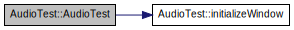
\includegraphics[width=350pt]{class_audio_test_a086084868d3cadb9b4c8e1a8549425e9_cgraph}
\end{center}
\end{figure}




\subsection{Member Function Documentation}
\hypertarget{class_audio_test_a9a38ae87dce3988e4560832475be32ca}{\index{Audio\-Test@{Audio\-Test}!create\-Audio\-Output@{create\-Audio\-Output}}
\index{create\-Audio\-Output@{create\-Audio\-Output}!AudioTest@{Audio\-Test}}
\subsubsection[{create\-Audio\-Output}]{\setlength{\rightskip}{0pt plus 5cm}void Audio\-Test\-::create\-Audio\-Output (
\begin{DoxyParamCaption}
{}
\end{DoxyParamCaption}
)\hspace{0.3cm}{\ttfamily [protected]}}}\label{class_audio_test_a9a38ae87dce3988e4560832475be32ca}
\hypertarget{class_audio_test_a80b6f4ce52947f96d9f243cf93d04a46}{\index{Audio\-Test@{Audio\-Test}!initialize\-Audio@{initialize\-Audio}}
\index{initialize\-Audio@{initialize\-Audio}!AudioTest@{Audio\-Test}}
\subsubsection[{initialize\-Audio}]{\setlength{\rightskip}{0pt plus 5cm}void Audio\-Test\-::initialize\-Audio (
\begin{DoxyParamCaption}
{}
\end{DoxyParamCaption}
)\hspace{0.3cm}{\ttfamily [protected]}}}\label{class_audio_test_a80b6f4ce52947f96d9f243cf93d04a46}
\hypertarget{class_audio_test_a1b80cfb92faf38273d77a908ad1ef803}{\index{Audio\-Test@{Audio\-Test}!initialize\-Window@{initialize\-Window}}
\index{initialize\-Window@{initialize\-Window}!AudioTest@{Audio\-Test}}
\subsubsection[{initialize\-Window}]{\setlength{\rightskip}{0pt plus 5cm}void Audio\-Test\-::initialize\-Window (
\begin{DoxyParamCaption}
{}
\end{DoxyParamCaption}
)\hspace{0.3cm}{\ttfamily [protected]}}}\label{class_audio_test_a1b80cfb92faf38273d77a908ad1ef803}
\begin{DoxyAttention}{Attention}
Consider moving this device finding to a non-\/graphical context 
\end{DoxyAttention}


Here is the caller graph for this function\-:
\nopagebreak
\begin{figure}[H]
\begin{center}
\leavevmode
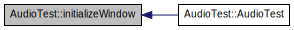
\includegraphics[width=350pt]{class_audio_test_a1b80cfb92faf38273d77a908ad1ef803_icgraph}
\end{center}
\end{figure}


\hypertarget{class_audio_test_a717dfe69311252d9890838a250946064}{\index{Audio\-Test@{Audio\-Test}!Setup@{Setup}}
\index{Setup@{Setup}!AudioTest@{Audio\-Test}}
\subsubsection[{Setup}]{\setlength{\rightskip}{0pt plus 5cm}void Audio\-Test\-::\-Setup (
\begin{DoxyParamCaption}
{}
\end{DoxyParamCaption}
)}}\label{class_audio_test_a717dfe69311252d9890838a250946064}


Here is the call graph for this function\-:
\nopagebreak
\begin{figure}[H]
\begin{center}
\leavevmode
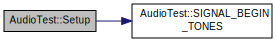
\includegraphics[width=348pt]{class_audio_test_a717dfe69311252d9890838a250946064_cgraph}
\end{center}
\end{figure}




Here is the caller graph for this function\-:\nopagebreak
\begin{figure}[H]
\begin{center}
\leavevmode
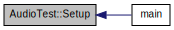
\includegraphics[width=246pt]{class_audio_test_a717dfe69311252d9890838a250946064_icgraph}
\end{center}
\end{figure}


\hypertarget{class_audio_test_a7f324e3db9ffe815a1c1b3af12e520a5}{\index{Audio\-Test@{Audio\-Test}!S\-I\-G\-N\-A\-L\-\_\-\-B\-E\-G\-I\-N\-\_\-\-C\-A\-P\-T\-U\-R\-E@{S\-I\-G\-N\-A\-L\-\_\-\-B\-E\-G\-I\-N\-\_\-\-C\-A\-P\-T\-U\-R\-E}}
\index{S\-I\-G\-N\-A\-L\-\_\-\-B\-E\-G\-I\-N\-\_\-\-C\-A\-P\-T\-U\-R\-E@{S\-I\-G\-N\-A\-L\-\_\-\-B\-E\-G\-I\-N\-\_\-\-C\-A\-P\-T\-U\-R\-E}!AudioTest@{Audio\-Test}}
\subsubsection[{S\-I\-G\-N\-A\-L\-\_\-\-B\-E\-G\-I\-N\-\_\-\-C\-A\-P\-T\-U\-R\-E}]{\setlength{\rightskip}{0pt plus 5cm}void Audio\-Test\-::\-S\-I\-G\-N\-A\-L\-\_\-\-B\-E\-G\-I\-N\-\_\-\-C\-A\-P\-T\-U\-R\-E (
\begin{DoxyParamCaption}
{}
\end{DoxyParamCaption}
)\hspace{0.3cm}{\ttfamily [signal]}}}\label{class_audio_test_a7f324e3db9ffe815a1c1b3af12e520a5}
\hypertarget{class_audio_test_a44db884ba0eaf1838099d0aeb29a04d6}{\index{Audio\-Test@{Audio\-Test}!S\-I\-G\-N\-A\-L\-\_\-\-B\-E\-G\-I\-N\-\_\-\-T\-O\-N\-E\-S@{S\-I\-G\-N\-A\-L\-\_\-\-B\-E\-G\-I\-N\-\_\-\-T\-O\-N\-E\-S}}
\index{S\-I\-G\-N\-A\-L\-\_\-\-B\-E\-G\-I\-N\-\_\-\-T\-O\-N\-E\-S@{S\-I\-G\-N\-A\-L\-\_\-\-B\-E\-G\-I\-N\-\_\-\-T\-O\-N\-E\-S}!AudioTest@{Audio\-Test}}
\subsubsection[{S\-I\-G\-N\-A\-L\-\_\-\-B\-E\-G\-I\-N\-\_\-\-T\-O\-N\-E\-S}]{\setlength{\rightskip}{0pt plus 5cm}void Audio\-Test\-::\-S\-I\-G\-N\-A\-L\-\_\-\-B\-E\-G\-I\-N\-\_\-\-T\-O\-N\-E\-S (
\begin{DoxyParamCaption}
{}
\end{DoxyParamCaption}
)\hspace{0.3cm}{\ttfamily [signal]}}}\label{class_audio_test_a44db884ba0eaf1838099d0aeb29a04d6}


Here is the caller graph for this function\-:
\nopagebreak
\begin{figure}[H]
\begin{center}
\leavevmode
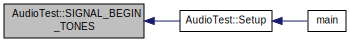
\includegraphics[width=350pt]{class_audio_test_a44db884ba0eaf1838099d0aeb29a04d6_icgraph}
\end{center}
\end{figure}


\hypertarget{class_audio_test_a97c30aeee89c952e4f9e213d26883da6}{\index{Audio\-Test@{Audio\-Test}!Volume\-Changed@{Volume\-Changed}}
\index{Volume\-Changed@{Volume\-Changed}!AudioTest@{Audio\-Test}}
\subsubsection[{Volume\-Changed}]{\setlength{\rightskip}{0pt plus 5cm}void Audio\-Test\-::\-Volume\-Changed (
\begin{DoxyParamCaption}
\item[{int}]{}
\end{DoxyParamCaption}
)\hspace{0.3cm}{\ttfamily [signal]}}}\label{class_audio_test_a97c30aeee89c952e4f9e213d26883da6}


\subsection{Member Data Documentation}
\hypertarget{class_audio_test_a96804bbcebef3ac9a5c2ce73d8ac2847}{\index{Audio\-Test@{Audio\-Test}!audio\-Graph@{audio\-Graph}}
\index{audio\-Graph@{audio\-Graph}!AudioTest@{Audio\-Test}}
\subsubsection[{audio\-Graph}]{\setlength{\rightskip}{0pt plus 5cm}{\bf Audio\-Graph}$\ast$ Audio\-Test\-::audio\-Graph\hspace{0.3cm}{\ttfamily [protected]}}}\label{class_audio_test_a96804bbcebef3ac9a5c2ce73d8ac2847}
\hypertarget{class_audio_test_af8f82fce5f5878c15a0c52e72a329f4c}{\index{Audio\-Test@{Audio\-Test}!audio\-Graph\-Window@{audio\-Graph\-Window}}
\index{audio\-Graph\-Window@{audio\-Graph\-Window}!AudioTest@{Audio\-Test}}
\subsubsection[{audio\-Graph\-Window}]{\setlength{\rightskip}{0pt plus 5cm}Q\-Main\-Window$\ast$ Audio\-Test\-::audio\-Graph\-Window\hspace{0.3cm}{\ttfamily [protected]}}}\label{class_audio_test_af8f82fce5f5878c15a0c52e72a329f4c}
\hypertarget{class_audio_test_acb4bb7befffd173d60885148b403d2fc}{\index{Audio\-Test@{Audio\-Test}!chart@{chart}}
\index{chart@{chart}!AudioTest@{Audio\-Test}}
\subsubsection[{chart}]{\setlength{\rightskip}{0pt plus 5cm}Q\-Chart$\ast$ Audio\-Test\-::chart\hspace{0.3cm}{\ttfamily [protected]}}}\label{class_audio_test_acb4bb7befffd173d60885148b403d2fc}
\hypertarget{class_audio_test_ac525335560da38c3d9a945f52d5c664f}{\index{Audio\-Test@{Audio\-Test}!chart\-View@{chart\-View}}
\index{chart\-View@{chart\-View}!AudioTest@{Audio\-Test}}
\subsubsection[{chart\-View}]{\setlength{\rightskip}{0pt plus 5cm}Q\-Chart\-View$\ast$ Audio\-Test\-::chart\-View\hspace{0.3cm}{\ttfamily [protected]}}}\label{class_audio_test_ac525335560da38c3d9a945f52d5c664f}
\hypertarget{class_audio_test_ae13d28e386d8b95cf2760194a3cee9cc}{\index{Audio\-Test@{Audio\-Test}!current\-Tone@{current\-Tone}}
\index{current\-Tone@{current\-Tone}!AudioTest@{Audio\-Test}}
\subsubsection[{current\-Tone}]{\setlength{\rightskip}{0pt plus 5cm}int Audio\-Test\-::current\-Tone\hspace{0.3cm}{\ttfamily [protected]}}}\label{class_audio_test_ae13d28e386d8b95cf2760194a3cee9cc}
\hypertarget{class_audio_test_a8ba597a8a62383d03f58710261771d4f}{\index{Audio\-Test@{Audio\-Test}!m\-\_\-base\-Frequency@{m\-\_\-base\-Frequency}}
\index{m\-\_\-base\-Frequency@{m\-\_\-base\-Frequency}!AudioTest@{Audio\-Test}}
\subsubsection[{m\-\_\-base\-Frequency}]{\setlength{\rightskip}{0pt plus 5cm}Q\-Spin\-Box$\ast$ Audio\-Test\-::m\-\_\-base\-Frequency\hspace{0.3cm}{\ttfamily [protected]}}}\label{class_audio_test_a8ba597a8a62383d03f58710261771d4f}
\hypertarget{class_audio_test_aab2b89738ef1f45c6e00387a54bdbfba}{\index{Audio\-Test@{Audio\-Test}!m\-\_\-base\-Frequency\-Label@{m\-\_\-base\-Frequency\-Label}}
\index{m\-\_\-base\-Frequency\-Label@{m\-\_\-base\-Frequency\-Label}!AudioTest@{Audio\-Test}}
\subsubsection[{m\-\_\-base\-Frequency\-Label}]{\setlength{\rightskip}{0pt plus 5cm}Q\-Label$\ast$ Audio\-Test\-::m\-\_\-base\-Frequency\-Label\hspace{0.3cm}{\ttfamily [protected]}}}\label{class_audio_test_aab2b89738ef1f45c6e00387a54bdbfba}
\hypertarget{class_audio_test_ab5999227ac75e0ecd7012e331ca36b2f}{\index{Audio\-Test@{Audio\-Test}!m\-\_\-frequency\-Slider@{m\-\_\-frequency\-Slider}}
\index{m\-\_\-frequency\-Slider@{m\-\_\-frequency\-Slider}!AudioTest@{Audio\-Test}}
\subsubsection[{m\-\_\-frequency\-Slider}]{\setlength{\rightskip}{0pt plus 5cm}Q\-Slider$\ast$ Audio\-Test\-::m\-\_\-frequency\-Slider\hspace{0.3cm}{\ttfamily [protected]}}}\label{class_audio_test_ab5999227ac75e0ecd7012e331ca36b2f}
\hypertarget{class_audio_test_a9da9104fab5169ae9016993136b22e2e}{\index{Audio\-Test@{Audio\-Test}!m\-\_\-network\-Device\-Box@{m\-\_\-network\-Device\-Box}}
\index{m\-\_\-network\-Device\-Box@{m\-\_\-network\-Device\-Box}!AudioTest@{Audio\-Test}}
\subsubsection[{m\-\_\-network\-Device\-Box}]{\setlength{\rightskip}{0pt plus 5cm}Q\-Combo\-Box$\ast$ Audio\-Test\-::m\-\_\-network\-Device\-Box\hspace{0.3cm}{\ttfamily [protected]}}}\label{class_audio_test_a9da9104fab5169ae9016993136b22e2e}
\hypertarget{class_audio_test_a845de1a2a2a6502d3e62dc6b2a7dae90}{\index{Audio\-Test@{Audio\-Test}!m\-\_\-number\-Of\-Tones@{m\-\_\-number\-Of\-Tones}}
\index{m\-\_\-number\-Of\-Tones@{m\-\_\-number\-Of\-Tones}!AudioTest@{Audio\-Test}}
\subsubsection[{m\-\_\-number\-Of\-Tones}]{\setlength{\rightskip}{0pt plus 5cm}Q\-Spin\-Box$\ast$ Audio\-Test\-::m\-\_\-number\-Of\-Tones\hspace{0.3cm}{\ttfamily [protected]}}}\label{class_audio_test_a845de1a2a2a6502d3e62dc6b2a7dae90}
\hypertarget{class_audio_test_a8c2e8d20ea6734c144cc2dac5c88a69e}{\index{Audio\-Test@{Audio\-Test}!m\-\_\-number\-Of\-Tones\-Label@{m\-\_\-number\-Of\-Tones\-Label}}
\index{m\-\_\-number\-Of\-Tones\-Label@{m\-\_\-number\-Of\-Tones\-Label}!AudioTest@{Audio\-Test}}
\subsubsection[{m\-\_\-number\-Of\-Tones\-Label}]{\setlength{\rightskip}{0pt plus 5cm}Q\-Label$\ast$ Audio\-Test\-::m\-\_\-number\-Of\-Tones\-Label\hspace{0.3cm}{\ttfamily [protected]}}}\label{class_audio_test_a8c2e8d20ea6734c144cc2dac5c88a69e}
\hypertarget{class_audio_test_a272651cef1e35ba3dae5bb3adffb5d76}{\index{Audio\-Test@{Audio\-Test}!m\-\_\-status\-Bar@{m\-\_\-status\-Bar}}
\index{m\-\_\-status\-Bar@{m\-\_\-status\-Bar}!AudioTest@{Audio\-Test}}
\subsubsection[{m\-\_\-status\-Bar}]{\setlength{\rightskip}{0pt plus 5cm}Q\-Status\-Bar$\ast$ Audio\-Test\-::m\-\_\-status\-Bar\hspace{0.3cm}{\ttfamily [protected]}}}\label{class_audio_test_a272651cef1e35ba3dae5bb3adffb5d76}
\hypertarget{class_audio_test_aaefe5dd3c1527190784ab1bfdc5abb22}{\index{Audio\-Test@{Audio\-Test}!m\-\_\-status\-Bar\-Label@{m\-\_\-status\-Bar\-Label}}
\index{m\-\_\-status\-Bar\-Label@{m\-\_\-status\-Bar\-Label}!AudioTest@{Audio\-Test}}
\subsubsection[{m\-\_\-status\-Bar\-Label}]{\setlength{\rightskip}{0pt plus 5cm}Q\-Label$\ast$ Audio\-Test\-::m\-\_\-status\-Bar\-Label\hspace{0.3cm}{\ttfamily [protected]}}}\label{class_audio_test_aaefe5dd3c1527190784ab1bfdc5abb22}
\hypertarget{class_audio_test_ac3f219c06b8fc68e769c52a0caba3c4a}{\index{Audio\-Test@{Audio\-Test}!m\-\_\-status\-Bar\-Label\-String@{m\-\_\-status\-Bar\-Label\-String}}
\index{m\-\_\-status\-Bar\-Label\-String@{m\-\_\-status\-Bar\-Label\-String}!AudioTest@{Audio\-Test}}
\subsubsection[{m\-\_\-status\-Bar\-Label\-String}]{\setlength{\rightskip}{0pt plus 5cm}Q\-String$\ast$ Audio\-Test\-::m\-\_\-status\-Bar\-Label\-String\hspace{0.3cm}{\ttfamily [protected]}}}\label{class_audio_test_ac3f219c06b8fc68e769c52a0caba3c4a}
\hypertarget{class_audio_test_a7cc252683f93e389b0783a8b34671665}{\index{Audio\-Test@{Audio\-Test}!m\-\_\-volume\-Label@{m\-\_\-volume\-Label}}
\index{m\-\_\-volume\-Label@{m\-\_\-volume\-Label}!AudioTest@{Audio\-Test}}
\subsubsection[{m\-\_\-volume\-Label}]{\setlength{\rightskip}{0pt plus 5cm}Q\-Label$\ast$ Audio\-Test\-::m\-\_\-volume\-Label\hspace{0.3cm}{\ttfamily [protected]}}}\label{class_audio_test_a7cc252683f93e389b0783a8b34671665}
\hypertarget{class_audio_test_a822b1b9f3ac4cd529e90187f713a0eb8}{\index{Audio\-Test@{Audio\-Test}!m\-\_\-volume\-Slider@{m\-\_\-volume\-Slider}}
\index{m\-\_\-volume\-Slider@{m\-\_\-volume\-Slider}!AudioTest@{Audio\-Test}}
\subsubsection[{m\-\_\-volume\-Slider}]{\setlength{\rightskip}{0pt plus 5cm}Q\-Slider$\ast$ Audio\-Test\-::m\-\_\-volume\-Slider\hspace{0.3cm}{\ttfamily [protected]}}}\label{class_audio_test_a822b1b9f3ac4cd529e90187f713a0eb8}
\hypertarget{class_audio_test_a1b07f5dd6e72a10b27065593c2b4adca}{\index{Audio\-Test@{Audio\-Test}!Packet\-Capture\-Thread@{Packet\-Capture\-Thread}}
\index{Packet\-Capture\-Thread@{Packet\-Capture\-Thread}!AudioTest@{Audio\-Test}}
\subsubsection[{Packet\-Capture\-Thread}]{\setlength{\rightskip}{0pt plus 5cm}Q\-Thread$\ast$ Audio\-Test\-::\-Packet\-Capture\-Thread\hspace{0.3cm}{\ttfamily [protected]}}}\label{class_audio_test_a1b07f5dd6e72a10b27065593c2b4adca}
\hypertarget{class_audio_test_a799c4ca17167556b33a0e863278717c0}{\index{Audio\-Test@{Audio\-Test}!pk@{pk}}
\index{pk@{pk}!AudioTest@{Audio\-Test}}
\subsubsection[{pk}]{\setlength{\rightskip}{0pt plus 5cm}{\bf Packet\-Capturer}$\ast$ Audio\-Test\-::pk\hspace{0.3cm}{\ttfamily [protected]}}}\label{class_audio_test_a799c4ca17167556b33a0e863278717c0}
\hypertarget{class_audio_test_a15e0d2b3243a7fa77753963084e23424}{\index{Audio\-Test@{Audio\-Test}!series@{series}}
\index{series@{series}!AudioTest@{Audio\-Test}}
\subsubsection[{series}]{\setlength{\rightskip}{0pt plus 5cm}Q\-Pie\-Series$\ast$ Audio\-Test\-::series\hspace{0.3cm}{\ttfamily [protected]}}}\label{class_audio_test_a15e0d2b3243a7fa77753963084e23424}
\hypertarget{class_audio_test_ab57b7deedbfb197745c28092e5c44fe7}{\index{Audio\-Test@{Audio\-Test}!slices@{slices}}
\index{slices@{slices}!AudioTest@{Audio\-Test}}
\subsubsection[{slices}]{\setlength{\rightskip}{0pt plus 5cm}Q\-Hash$<$int, Q\-Pie\-Slice$\ast$$>$ Audio\-Test\-::slices\hspace{0.3cm}{\ttfamily [protected]}}}\label{class_audio_test_ab57b7deedbfb197745c28092e5c44fe7}
\hypertarget{class_audio_test_a3f926ca4bd5cd5a38794db6b85a832dd}{\index{Audio\-Test@{Audio\-Test}!tone\-Manager@{tone\-Manager}}
\index{tone\-Manager@{tone\-Manager}!AudioTest@{Audio\-Test}}
\subsubsection[{tone\-Manager}]{\setlength{\rightskip}{0pt plus 5cm}{\bf Tone\-Manager}$\ast$ Audio\-Test\-::tone\-Manager\hspace{0.3cm}{\ttfamily [protected]}}}\label{class_audio_test_a3f926ca4bd5cd5a38794db6b85a832dd}
\hypertarget{class_audio_test_a9c61f6a4dd4d0a6947d2a1a52d9df431}{\index{Audio\-Test@{Audio\-Test}!Tone\-Manager\-Thread@{Tone\-Manager\-Thread}}
\index{Tone\-Manager\-Thread@{Tone\-Manager\-Thread}!AudioTest@{Audio\-Test}}
\subsubsection[{Tone\-Manager\-Thread}]{\setlength{\rightskip}{0pt plus 5cm}Q\-Thread$\ast$ Audio\-Test\-::\-Tone\-Manager\-Thread\hspace{0.3cm}{\ttfamily [protected]}}}\label{class_audio_test_a9c61f6a4dd4d0a6947d2a1a52d9df431}


The documentation for this class was generated from the following files\-:\begin{DoxyCompactItemize}
\item 
Network-\/\-Music/\hyperlink{audiooutput_8h}{audiooutput.\-h}\item 
Network-\/\-Music/\hyperlink{audiooutput_8cpp}{audiooutput.\-cpp}\end{DoxyCompactItemize}

\hypertarget{class_generator}{\section{Generator Class Reference}
\label{class_generator}\index{Generator@{Generator}}
}


{\ttfamily \#include $<$generator.\-h$>$}

\subsection*{Public Member Functions}
\begin{DoxyCompactItemize}
\item 
\hyperlink{class_generator_ac70583c21208d97c0474d9ab23f69a2b}{Generator} (const Q\-Audio\-Format \&format, qint64 duration\-Us, int sample\-Rate, Q\-Object $\ast$parent)
\item 
\hyperlink{class_generator_acc85fbe22690003267ba899bacf777d1}{$\sim$\-Generator} ()
\item 
void \hyperlink{class_generator_a3f0bc6d7fed7eaf8d497d3e50149982b}{start} ()
\item 
void \hyperlink{class_generator_a698e9aa26989e005a709c297ebea3492}{stop} ()
\item 
void \hyperlink{class_generator_a54a730f69fe887837f3f83080e32201f}{set\-Frequency} (int value)
\item 
qint64 \hyperlink{class_generator_ada073b90efc5104c049eef04844c8801}{Get\-Pos} ()
\item 
void \hyperlink{class_generator_a9aa165c8eca0883e9792d63153701f49}{Set\-Pos} (qint64 val)
\item 
qint64 \hyperlink{class_generator_ac818d4583f77c0f29bbeafbb31995ff8}{read\-Data} (char $\ast$data, qint64 maxlen)
\item 
qint64 \hyperlink{class_generator_a16d82d88527ec5a0be4052b13d63417a}{write\-Data} (const char $\ast$data, qint64 len)
\item 
qint64 \hyperlink{class_generator_ab06a2f7a10bdcf3edd3fd0a11ac6d53f}{bytes\-Available} () const 
\end{DoxyCompactItemize}
\subsection*{Static Public Member Functions}
\begin{DoxyCompactItemize}
\item 
static Q\-Byte\-Array $\ast$ \hyperlink{class_generator_abaee73437c469e40bf5d7c0c15bdc48f}{Generate\-Data} (const Q\-Audio\-Format \&format, qint64 frequency)
\end{DoxyCompactItemize}
\subsection*{Public Attributes}
\begin{DoxyCompactItemize}
\item 
Q\-Byte\-Array $\ast$ \hyperlink{class_generator_ac7d96c5f663351ce95f3e1cf9a862e00}{m\-\_\-buffer}
\item 
qint64 \hyperlink{class_generator_aa718042777706f4e9ee2ab302d0e4071}{m\-\_\-pos}
\end{DoxyCompactItemize}


\subsection{Constructor \& Destructor Documentation}
\hypertarget{class_generator_ac70583c21208d97c0474d9ab23f69a2b}{\index{Generator@{Generator}!Generator@{Generator}}
\index{Generator@{Generator}!Generator@{Generator}}
\subsubsection[{Generator}]{\setlength{\rightskip}{0pt plus 5cm}Generator\-::\-Generator (
\begin{DoxyParamCaption}
\item[{const Q\-Audio\-Format \&}]{format, }
\item[{qint64}]{duration\-Us, }
\item[{int}]{sample\-Rate, }
\item[{Q\-Object $\ast$}]{parent}
\end{DoxyParamCaption}
)}}\label{class_generator_ac70583c21208d97c0474d9ab23f69a2b}
Acts as a file type device to get audio from \hypertarget{class_generator_acc85fbe22690003267ba899bacf777d1}{\index{Generator@{Generator}!$\sim$\-Generator@{$\sim$\-Generator}}
\index{$\sim$\-Generator@{$\sim$\-Generator}!Generator@{Generator}}
\subsubsection[{$\sim$\-Generator}]{\setlength{\rightskip}{0pt plus 5cm}Generator\-::$\sim$\-Generator (
\begin{DoxyParamCaption}
{}
\end{DoxyParamCaption}
)}}\label{class_generator_acc85fbe22690003267ba899bacf777d1}


\subsection{Member Function Documentation}
\hypertarget{class_generator_ab06a2f7a10bdcf3edd3fd0a11ac6d53f}{\index{Generator@{Generator}!bytes\-Available@{bytes\-Available}}
\index{bytes\-Available@{bytes\-Available}!Generator@{Generator}}
\subsubsection[{bytes\-Available}]{\setlength{\rightskip}{0pt plus 5cm}qint64 Generator\-::bytes\-Available (
\begin{DoxyParamCaption}
{}
\end{DoxyParamCaption}
) const}}\label{class_generator_ab06a2f7a10bdcf3edd3fd0a11ac6d53f}
\hypertarget{class_generator_abaee73437c469e40bf5d7c0c15bdc48f}{\index{Generator@{Generator}!Generate\-Data@{Generate\-Data}}
\index{Generate\-Data@{Generate\-Data}!Generator@{Generator}}
\subsubsection[{Generate\-Data}]{\setlength{\rightskip}{0pt plus 5cm}Q\-Byte\-Array $\ast$ Generator\-::\-Generate\-Data (
\begin{DoxyParamCaption}
\item[{const Q\-Audio\-Format \&}]{format, }
\item[{qint64}]{frequency}
\end{DoxyParamCaption}
)\hspace{0.3cm}{\ttfamily [static]}}}\label{class_generator_abaee73437c469e40bf5d7c0c15bdc48f}


Here is the caller graph for this function\-:
\nopagebreak
\begin{figure}[H]
\begin{center}
\leavevmode
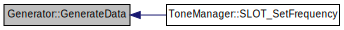
\includegraphics[width=350pt]{class_generator_abaee73437c469e40bf5d7c0c15bdc48f_icgraph}
\end{center}
\end{figure}


\hypertarget{class_generator_ada073b90efc5104c049eef04844c8801}{\index{Generator@{Generator}!Get\-Pos@{Get\-Pos}}
\index{Get\-Pos@{Get\-Pos}!Generator@{Generator}}
\subsubsection[{Get\-Pos}]{\setlength{\rightskip}{0pt plus 5cm}qint64 Generator\-::\-Get\-Pos (
\begin{DoxyParamCaption}
{}
\end{DoxyParamCaption}
)}}\label{class_generator_ada073b90efc5104c049eef04844c8801}


Here is the caller graph for this function\-:\nopagebreak
\begin{figure}[H]
\begin{center}
\leavevmode
\includegraphics[width=314pt]{class_generator_ada073b90efc5104c049eef04844c8801_icgraph}
\end{center}
\end{figure}


\hypertarget{class_generator_ac818d4583f77c0f29bbeafbb31995ff8}{\index{Generator@{Generator}!read\-Data@{read\-Data}}
\index{read\-Data@{read\-Data}!Generator@{Generator}}
\subsubsection[{read\-Data}]{\setlength{\rightskip}{0pt plus 5cm}qint64 Generator\-::read\-Data (
\begin{DoxyParamCaption}
\item[{char $\ast$}]{data, }
\item[{qint64}]{maxlen}
\end{DoxyParamCaption}
)}}\label{class_generator_ac818d4583f77c0f29bbeafbb31995ff8}
\hypertarget{class_generator_a54a730f69fe887837f3f83080e32201f}{\index{Generator@{Generator}!set\-Frequency@{set\-Frequency}}
\index{set\-Frequency@{set\-Frequency}!Generator@{Generator}}
\subsubsection[{set\-Frequency}]{\setlength{\rightskip}{0pt plus 5cm}void Generator\-::set\-Frequency (
\begin{DoxyParamCaption}
\item[{int}]{value}
\end{DoxyParamCaption}
)}}\label{class_generator_a54a730f69fe887837f3f83080e32201f}
\hypertarget{class_generator_a9aa165c8eca0883e9792d63153701f49}{\index{Generator@{Generator}!Set\-Pos@{Set\-Pos}}
\index{Set\-Pos@{Set\-Pos}!Generator@{Generator}}
\subsubsection[{Set\-Pos}]{\setlength{\rightskip}{0pt plus 5cm}void Generator\-::\-Set\-Pos (
\begin{DoxyParamCaption}
\item[{qint64}]{val}
\end{DoxyParamCaption}
)}}\label{class_generator_a9aa165c8eca0883e9792d63153701f49}


Here is the caller graph for this function\-:\nopagebreak
\begin{figure}[H]
\begin{center}
\leavevmode
\includegraphics[width=314pt]{class_generator_a9aa165c8eca0883e9792d63153701f49_icgraph}
\end{center}
\end{figure}


\hypertarget{class_generator_a3f0bc6d7fed7eaf8d497d3e50149982b}{\index{Generator@{Generator}!start@{start}}
\index{start@{start}!Generator@{Generator}}
\subsubsection[{start}]{\setlength{\rightskip}{0pt plus 5cm}void Generator\-::start (
\begin{DoxyParamCaption}
{}
\end{DoxyParamCaption}
)}}\label{class_generator_a3f0bc6d7fed7eaf8d497d3e50149982b}


Here is the caller graph for this function\-:\nopagebreak
\begin{figure}[H]
\begin{center}
\leavevmode
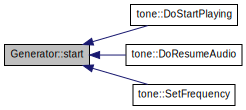
\includegraphics[width=318pt]{class_generator_a3f0bc6d7fed7eaf8d497d3e50149982b_icgraph}
\end{center}
\end{figure}


\hypertarget{class_generator_a698e9aa26989e005a709c297ebea3492}{\index{Generator@{Generator}!stop@{stop}}
\index{stop@{stop}!Generator@{Generator}}
\subsubsection[{stop}]{\setlength{\rightskip}{0pt plus 5cm}void Generator\-::stop (
\begin{DoxyParamCaption}
{}
\end{DoxyParamCaption}
)}}\label{class_generator_a698e9aa26989e005a709c297ebea3492}
\hypertarget{class_generator_a16d82d88527ec5a0be4052b13d63417a}{\index{Generator@{Generator}!write\-Data@{write\-Data}}
\index{write\-Data@{write\-Data}!Generator@{Generator}}
\subsubsection[{write\-Data}]{\setlength{\rightskip}{0pt plus 5cm}qint64 Generator\-::write\-Data (
\begin{DoxyParamCaption}
\item[{const char $\ast$}]{data, }
\item[{qint64}]{len}
\end{DoxyParamCaption}
)}}\label{class_generator_a16d82d88527ec5a0be4052b13d63417a}


\subsection{Member Data Documentation}
\hypertarget{class_generator_ac7d96c5f663351ce95f3e1cf9a862e00}{\index{Generator@{Generator}!m\-\_\-buffer@{m\-\_\-buffer}}
\index{m\-\_\-buffer@{m\-\_\-buffer}!Generator@{Generator}}
\subsubsection[{m\-\_\-buffer}]{\setlength{\rightskip}{0pt plus 5cm}Q\-Byte\-Array$\ast$ Generator\-::m\-\_\-buffer}}\label{class_generator_ac7d96c5f663351ce95f3e1cf9a862e00}
\hypertarget{class_generator_aa718042777706f4e9ee2ab302d0e4071}{\index{Generator@{Generator}!m\-\_\-pos@{m\-\_\-pos}}
\index{m\-\_\-pos@{m\-\_\-pos}!Generator@{Generator}}
\subsubsection[{m\-\_\-pos}]{\setlength{\rightskip}{0pt plus 5cm}qint64 Generator\-::m\-\_\-pos}}\label{class_generator_aa718042777706f4e9ee2ab302d0e4071}


The documentation for this class was generated from the following files\-:\begin{DoxyCompactItemize}
\item 
Network-\/\-Music/\hyperlink{generator_8h}{generator.\-h}\item 
Network-\/\-Music/\hyperlink{generator_8cpp}{generator.\-cpp}\end{DoxyCompactItemize}

\input{class_main_window}
\hypertarget{class_packet_capturer}{\section{Packet\-Capturer Class Reference}
\label{class_packet_capturer}\index{Packet\-Capturer@{Packet\-Capturer}}
}


{\ttfamily \#include $<$packetcapturer.\-h$>$}

\subsection*{Public Slots}
\begin{DoxyCompactItemize}
\item 
void \hyperlink{class_packet_capturer_a3f008c97baedf3417013623b05b0de34}{S\-L\-O\-T\-\_\-\-C\-A\-P\-T\-U\-R\-E} ()
\end{DoxyCompactItemize}
\subsection*{Signals}
\begin{DoxyCompactItemize}
\item 
void \hyperlink{class_packet_capturer_a010699f00f58d9135c95eb358e40889b}{S\-I\-G\-\_\-\-N\-E\-W\-\_\-\-T\-O\-N\-E} (int, int)
\end{DoxyCompactItemize}
\subsection*{Public Member Functions}
\begin{DoxyCompactItemize}
\item 
\hyperlink{class_packet_capturer_a9318e16609d0662061b09e4f80984160}{Packet\-Capturer} (Q\-Object $\ast$parent=0)
\item 
\hyperlink{class_packet_capturer_a39bf6aec9827c081c90f90facc428a26}{Packet\-Capturer} (const char $\ast$device\-Name)
\item 
void \hyperlink{class_packet_capturer_a4df4e57d6ad6d62bf48f3e7a421a98d0}{Change\-Emitter} (int value, int often)
\item 
\hyperlink{class_packet_capturer_af5e2c8ad13949df4673c675a05e50219}{$\sim$\-Packet\-Capturer} ()
\end{DoxyCompactItemize}


\subsection{Constructor \& Destructor Documentation}
\hypertarget{class_packet_capturer_a9318e16609d0662061b09e4f80984160}{\index{Packet\-Capturer@{Packet\-Capturer}!Packet\-Capturer@{Packet\-Capturer}}
\index{Packet\-Capturer@{Packet\-Capturer}!PacketCapturer@{Packet\-Capturer}}
\subsubsection[{Packet\-Capturer}]{\setlength{\rightskip}{0pt plus 5cm}Packet\-Capturer\-::\-Packet\-Capturer (
\begin{DoxyParamCaption}
\item[{Q\-Object $\ast$}]{parent = {\ttfamily 0}}
\end{DoxyParamCaption}
)\hspace{0.3cm}{\ttfamily [explicit]}}}\label{class_packet_capturer_a9318e16609d0662061b09e4f80984160}
\hypertarget{class_packet_capturer_a39bf6aec9827c081c90f90facc428a26}{\index{Packet\-Capturer@{Packet\-Capturer}!Packet\-Capturer@{Packet\-Capturer}}
\index{Packet\-Capturer@{Packet\-Capturer}!PacketCapturer@{Packet\-Capturer}}
\subsubsection[{Packet\-Capturer}]{\setlength{\rightskip}{0pt plus 5cm}Packet\-Capturer\-::\-Packet\-Capturer (
\begin{DoxyParamCaption}
\item[{const char $\ast$}]{device\-Name}
\end{DoxyParamCaption}
)}}\label{class_packet_capturer_a39bf6aec9827c081c90f90facc428a26}
\begin{DoxyNote}{Note}
seems like a bad design but it works 
\end{DoxyNote}
\hypertarget{class_packet_capturer_af5e2c8ad13949df4673c675a05e50219}{\index{Packet\-Capturer@{Packet\-Capturer}!$\sim$\-Packet\-Capturer@{$\sim$\-Packet\-Capturer}}
\index{$\sim$\-Packet\-Capturer@{$\sim$\-Packet\-Capturer}!PacketCapturer@{Packet\-Capturer}}
\subsubsection[{$\sim$\-Packet\-Capturer}]{\setlength{\rightskip}{0pt plus 5cm}Packet\-Capturer\-::$\sim$\-Packet\-Capturer (
\begin{DoxyParamCaption}
{}
\end{DoxyParamCaption}
)}}\label{class_packet_capturer_af5e2c8ad13949df4673c675a05e50219}


\subsection{Member Function Documentation}
\hypertarget{class_packet_capturer_a4df4e57d6ad6d62bf48f3e7a421a98d0}{\index{Packet\-Capturer@{Packet\-Capturer}!Change\-Emitter@{Change\-Emitter}}
\index{Change\-Emitter@{Change\-Emitter}!PacketCapturer@{Packet\-Capturer}}
\subsubsection[{Change\-Emitter}]{\setlength{\rightskip}{0pt plus 5cm}void Packet\-Capturer\-::\-Change\-Emitter (
\begin{DoxyParamCaption}
\item[{int}]{value, }
\item[{int}]{often}
\end{DoxyParamCaption}
)}}\label{class_packet_capturer_a4df4e57d6ad6d62bf48f3e7a421a98d0}


Here is the call graph for this function\-:
\nopagebreak
\begin{figure}[H]
\begin{center}
\leavevmode
\includegraphics[width=350pt]{class_packet_capturer_a4df4e57d6ad6d62bf48f3e7a421a98d0_cgraph}
\end{center}
\end{figure}




Here is the caller graph for this function\-:
\nopagebreak
\begin{figure}[H]
\begin{center}
\leavevmode
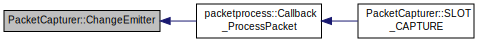
\includegraphics[width=350pt]{class_packet_capturer_a4df4e57d6ad6d62bf48f3e7a421a98d0_icgraph}
\end{center}
\end{figure}


\hypertarget{class_packet_capturer_a010699f00f58d9135c95eb358e40889b}{\index{Packet\-Capturer@{Packet\-Capturer}!S\-I\-G\-\_\-\-N\-E\-W\-\_\-\-T\-O\-N\-E@{S\-I\-G\-\_\-\-N\-E\-W\-\_\-\-T\-O\-N\-E}}
\index{S\-I\-G\-\_\-\-N\-E\-W\-\_\-\-T\-O\-N\-E@{S\-I\-G\-\_\-\-N\-E\-W\-\_\-\-T\-O\-N\-E}!PacketCapturer@{Packet\-Capturer}}
\subsubsection[{S\-I\-G\-\_\-\-N\-E\-W\-\_\-\-T\-O\-N\-E}]{\setlength{\rightskip}{0pt plus 5cm}void Packet\-Capturer\-::\-S\-I\-G\-\_\-\-N\-E\-W\-\_\-\-T\-O\-N\-E (
\begin{DoxyParamCaption}
\item[{int}]{, }
\item[{int}]{}
\end{DoxyParamCaption}
)\hspace{0.3cm}{\ttfamily [signal]}}}\label{class_packet_capturer_a010699f00f58d9135c95eb358e40889b}


Here is the caller graph for this function\-:
\nopagebreak
\begin{figure}[H]
\begin{center}
\leavevmode
\includegraphics[width=350pt]{class_packet_capturer_a010699f00f58d9135c95eb358e40889b_icgraph}
\end{center}
\end{figure}


\hypertarget{class_packet_capturer_a3f008c97baedf3417013623b05b0de34}{\index{Packet\-Capturer@{Packet\-Capturer}!S\-L\-O\-T\-\_\-\-C\-A\-P\-T\-U\-R\-E@{S\-L\-O\-T\-\_\-\-C\-A\-P\-T\-U\-R\-E}}
\index{S\-L\-O\-T\-\_\-\-C\-A\-P\-T\-U\-R\-E@{S\-L\-O\-T\-\_\-\-C\-A\-P\-T\-U\-R\-E}!PacketCapturer@{Packet\-Capturer}}
\subsubsection[{S\-L\-O\-T\-\_\-\-C\-A\-P\-T\-U\-R\-E}]{\setlength{\rightskip}{0pt plus 5cm}void Packet\-Capturer\-::\-S\-L\-O\-T\-\_\-\-C\-A\-P\-T\-U\-R\-E (
\begin{DoxyParamCaption}
{}
\end{DoxyParamCaption}
)\hspace{0.3cm}{\ttfamily [slot]}}}\label{class_packet_capturer_a3f008c97baedf3417013623b05b0de34}


Here is the call graph for this function\-:
\nopagebreak
\begin{figure}[H]
\begin{center}
\leavevmode
\includegraphics[width=350pt]{class_packet_capturer_a3f008c97baedf3417013623b05b0de34_cgraph}
\end{center}
\end{figure}




The documentation for this class was generated from the following files\-:\begin{DoxyCompactItemize}
\item 
Network-\/\-Music/\hyperlink{packetcapturer_8h}{packetcapturer.\-h}\item 
Network-\/\-Music/\hyperlink{packetcapturer_8cpp}{packetcapturer.\-cpp}\end{DoxyCompactItemize}

\hypertarget{structpacketprocess_1_1sniff__ethernet}{\section{packetprocess\-:\-:sniff\-\_\-ethernet Struct Reference}
\label{structpacketprocess_1_1sniff__ethernet}\index{packetprocess\-::sniff\-\_\-ethernet@{packetprocess\-::sniff\-\_\-ethernet}}
}
\subsection*{Public Attributes}
\begin{DoxyCompactItemize}
\item 
u\-\_\-char \hyperlink{structpacketprocess_1_1sniff__ethernet_a85e01cf751d0684915d6cd4502b476bc}{ether\-\_\-dhost} \mbox{[}E\-T\-H\-E\-R\-\_\-\-A\-D\-D\-R\-\_\-\-L\-E\-N\mbox{]}
\item 
u\-\_\-char \hyperlink{structpacketprocess_1_1sniff__ethernet_a7fd15b2b34d9dfb673740d90ef101dc8}{ether\-\_\-shost} \mbox{[}E\-T\-H\-E\-R\-\_\-\-A\-D\-D\-R\-\_\-\-L\-E\-N\mbox{]}
\item 
u\-\_\-short \hyperlink{structpacketprocess_1_1sniff__ethernet_ac4e709a11c8035f019c15e21dbb8595f}{ether\-\_\-type}
\end{DoxyCompactItemize}


\subsection{Member Data Documentation}
\hypertarget{structpacketprocess_1_1sniff__ethernet_a85e01cf751d0684915d6cd4502b476bc}{\index{packetprocess\-::sniff\-\_\-ethernet@{packetprocess\-::sniff\-\_\-ethernet}!ether\-\_\-dhost@{ether\-\_\-dhost}}
\index{ether\-\_\-dhost@{ether\-\_\-dhost}!packetprocess::sniff_ethernet@{packetprocess\-::sniff\-\_\-ethernet}}
\subsubsection[{ether\-\_\-dhost}]{\setlength{\rightskip}{0pt plus 5cm}u\-\_\-char packetprocess\-::sniff\-\_\-ethernet\-::ether\-\_\-dhost\mbox{[}E\-T\-H\-E\-R\-\_\-\-A\-D\-D\-R\-\_\-\-L\-E\-N\mbox{]}}}\label{structpacketprocess_1_1sniff__ethernet_a85e01cf751d0684915d6cd4502b476bc}
\hypertarget{structpacketprocess_1_1sniff__ethernet_a7fd15b2b34d9dfb673740d90ef101dc8}{\index{packetprocess\-::sniff\-\_\-ethernet@{packetprocess\-::sniff\-\_\-ethernet}!ether\-\_\-shost@{ether\-\_\-shost}}
\index{ether\-\_\-shost@{ether\-\_\-shost}!packetprocess::sniff_ethernet@{packetprocess\-::sniff\-\_\-ethernet}}
\subsubsection[{ether\-\_\-shost}]{\setlength{\rightskip}{0pt plus 5cm}u\-\_\-char packetprocess\-::sniff\-\_\-ethernet\-::ether\-\_\-shost\mbox{[}E\-T\-H\-E\-R\-\_\-\-A\-D\-D\-R\-\_\-\-L\-E\-N\mbox{]}}}\label{structpacketprocess_1_1sniff__ethernet_a7fd15b2b34d9dfb673740d90ef101dc8}
\hypertarget{structpacketprocess_1_1sniff__ethernet_ac4e709a11c8035f019c15e21dbb8595f}{\index{packetprocess\-::sniff\-\_\-ethernet@{packetprocess\-::sniff\-\_\-ethernet}!ether\-\_\-type@{ether\-\_\-type}}
\index{ether\-\_\-type@{ether\-\_\-type}!packetprocess::sniff_ethernet@{packetprocess\-::sniff\-\_\-ethernet}}
\subsubsection[{ether\-\_\-type}]{\setlength{\rightskip}{0pt plus 5cm}u\-\_\-short packetprocess\-::sniff\-\_\-ethernet\-::ether\-\_\-type}}\label{structpacketprocess_1_1sniff__ethernet_ac4e709a11c8035f019c15e21dbb8595f}


The documentation for this struct was generated from the following file\-:\begin{DoxyCompactItemize}
\item 
Network-\/\-Music/\hyperlink{packetcapturer_8cpp}{packetcapturer.\-cpp}\end{DoxyCompactItemize}

\hypertarget{structpacketprocess_1_1sniff__ip}{\section{packetprocess\-:\-:sniff\-\_\-ip Struct Reference}
\label{structpacketprocess_1_1sniff__ip}\index{packetprocess\-::sniff\-\_\-ip@{packetprocess\-::sniff\-\_\-ip}}
}
\subsection*{Public Attributes}
\begin{DoxyCompactItemize}
\item 
u\-\_\-char \hyperlink{structpacketprocess_1_1sniff__ip_a58f9c8e74a6204cd38bb6e404c2338c5}{ip\-\_\-vhl}
\item 
u\-\_\-char \hyperlink{structpacketprocess_1_1sniff__ip_a106bc8a251b55cdd13934bfed4785ae6}{ip\-\_\-tos}
\item 
u\-\_\-short \hyperlink{structpacketprocess_1_1sniff__ip_a98befd872cec3609b97989647cf5f9fd}{ip\-\_\-len}
\item 
u\-\_\-short \hyperlink{structpacketprocess_1_1sniff__ip_aa756a51f634dc93175521ea1d58ed36c}{ip\-\_\-id}
\item 
u\-\_\-short \hyperlink{structpacketprocess_1_1sniff__ip_a63728e3756b9d6736049dbed1b189275}{ip\-\_\-off}
\item 
u\-\_\-char \hyperlink{structpacketprocess_1_1sniff__ip_adcc8fd2d0bc337b78d7956e150bd5d89}{ip\-\_\-ttl}
\item 
u\-\_\-char \hyperlink{structpacketprocess_1_1sniff__ip_a98e71ce9ec87082492b4bf2622903ae3}{ip\-\_\-p}
\item 
u\-\_\-short \hyperlink{structpacketprocess_1_1sniff__ip_a596850a71ac22e40f393d5ea7d456b1e}{ip\-\_\-sum}
\item 
struct in\-\_\-addr ip\-\_\-src \hyperlink{structpacketprocess_1_1sniff__ip_ac400f30b4020540644d08fedaa2349f2}{ip\-\_\-dst}
\end{DoxyCompactItemize}


\subsection{Member Data Documentation}
\hypertarget{structpacketprocess_1_1sniff__ip_ac400f30b4020540644d08fedaa2349f2}{\index{packetprocess\-::sniff\-\_\-ip@{packetprocess\-::sniff\-\_\-ip}!ip\-\_\-dst@{ip\-\_\-dst}}
\index{ip\-\_\-dst@{ip\-\_\-dst}!packetprocess::sniff_ip@{packetprocess\-::sniff\-\_\-ip}}
\subsubsection[{ip\-\_\-dst}]{\setlength{\rightskip}{0pt plus 5cm}struct in\-\_\-addr ip\-\_\-src packetprocess\-::sniff\-\_\-ip\-::ip\-\_\-dst}}\label{structpacketprocess_1_1sniff__ip_ac400f30b4020540644d08fedaa2349f2}
\hypertarget{structpacketprocess_1_1sniff__ip_aa756a51f634dc93175521ea1d58ed36c}{\index{packetprocess\-::sniff\-\_\-ip@{packetprocess\-::sniff\-\_\-ip}!ip\-\_\-id@{ip\-\_\-id}}
\index{ip\-\_\-id@{ip\-\_\-id}!packetprocess::sniff_ip@{packetprocess\-::sniff\-\_\-ip}}
\subsubsection[{ip\-\_\-id}]{\setlength{\rightskip}{0pt plus 5cm}u\-\_\-short packetprocess\-::sniff\-\_\-ip\-::ip\-\_\-id}}\label{structpacketprocess_1_1sniff__ip_aa756a51f634dc93175521ea1d58ed36c}
\hypertarget{structpacketprocess_1_1sniff__ip_a98befd872cec3609b97989647cf5f9fd}{\index{packetprocess\-::sniff\-\_\-ip@{packetprocess\-::sniff\-\_\-ip}!ip\-\_\-len@{ip\-\_\-len}}
\index{ip\-\_\-len@{ip\-\_\-len}!packetprocess::sniff_ip@{packetprocess\-::sniff\-\_\-ip}}
\subsubsection[{ip\-\_\-len}]{\setlength{\rightskip}{0pt plus 5cm}u\-\_\-short packetprocess\-::sniff\-\_\-ip\-::ip\-\_\-len}}\label{structpacketprocess_1_1sniff__ip_a98befd872cec3609b97989647cf5f9fd}
\hypertarget{structpacketprocess_1_1sniff__ip_a63728e3756b9d6736049dbed1b189275}{\index{packetprocess\-::sniff\-\_\-ip@{packetprocess\-::sniff\-\_\-ip}!ip\-\_\-off@{ip\-\_\-off}}
\index{ip\-\_\-off@{ip\-\_\-off}!packetprocess::sniff_ip@{packetprocess\-::sniff\-\_\-ip}}
\subsubsection[{ip\-\_\-off}]{\setlength{\rightskip}{0pt plus 5cm}u\-\_\-short packetprocess\-::sniff\-\_\-ip\-::ip\-\_\-off}}\label{structpacketprocess_1_1sniff__ip_a63728e3756b9d6736049dbed1b189275}
\hypertarget{structpacketprocess_1_1sniff__ip_a98e71ce9ec87082492b4bf2622903ae3}{\index{packetprocess\-::sniff\-\_\-ip@{packetprocess\-::sniff\-\_\-ip}!ip\-\_\-p@{ip\-\_\-p}}
\index{ip\-\_\-p@{ip\-\_\-p}!packetprocess::sniff_ip@{packetprocess\-::sniff\-\_\-ip}}
\subsubsection[{ip\-\_\-p}]{\setlength{\rightskip}{0pt plus 5cm}u\-\_\-char packetprocess\-::sniff\-\_\-ip\-::ip\-\_\-p}}\label{structpacketprocess_1_1sniff__ip_a98e71ce9ec87082492b4bf2622903ae3}
\hypertarget{structpacketprocess_1_1sniff__ip_a596850a71ac22e40f393d5ea7d456b1e}{\index{packetprocess\-::sniff\-\_\-ip@{packetprocess\-::sniff\-\_\-ip}!ip\-\_\-sum@{ip\-\_\-sum}}
\index{ip\-\_\-sum@{ip\-\_\-sum}!packetprocess::sniff_ip@{packetprocess\-::sniff\-\_\-ip}}
\subsubsection[{ip\-\_\-sum}]{\setlength{\rightskip}{0pt plus 5cm}u\-\_\-short packetprocess\-::sniff\-\_\-ip\-::ip\-\_\-sum}}\label{structpacketprocess_1_1sniff__ip_a596850a71ac22e40f393d5ea7d456b1e}
\hypertarget{structpacketprocess_1_1sniff__ip_a106bc8a251b55cdd13934bfed4785ae6}{\index{packetprocess\-::sniff\-\_\-ip@{packetprocess\-::sniff\-\_\-ip}!ip\-\_\-tos@{ip\-\_\-tos}}
\index{ip\-\_\-tos@{ip\-\_\-tos}!packetprocess::sniff_ip@{packetprocess\-::sniff\-\_\-ip}}
\subsubsection[{ip\-\_\-tos}]{\setlength{\rightskip}{0pt plus 5cm}u\-\_\-char packetprocess\-::sniff\-\_\-ip\-::ip\-\_\-tos}}\label{structpacketprocess_1_1sniff__ip_a106bc8a251b55cdd13934bfed4785ae6}
\hypertarget{structpacketprocess_1_1sniff__ip_adcc8fd2d0bc337b78d7956e150bd5d89}{\index{packetprocess\-::sniff\-\_\-ip@{packetprocess\-::sniff\-\_\-ip}!ip\-\_\-ttl@{ip\-\_\-ttl}}
\index{ip\-\_\-ttl@{ip\-\_\-ttl}!packetprocess::sniff_ip@{packetprocess\-::sniff\-\_\-ip}}
\subsubsection[{ip\-\_\-ttl}]{\setlength{\rightskip}{0pt plus 5cm}u\-\_\-char packetprocess\-::sniff\-\_\-ip\-::ip\-\_\-ttl}}\label{structpacketprocess_1_1sniff__ip_adcc8fd2d0bc337b78d7956e150bd5d89}
\hypertarget{structpacketprocess_1_1sniff__ip_a58f9c8e74a6204cd38bb6e404c2338c5}{\index{packetprocess\-::sniff\-\_\-ip@{packetprocess\-::sniff\-\_\-ip}!ip\-\_\-vhl@{ip\-\_\-vhl}}
\index{ip\-\_\-vhl@{ip\-\_\-vhl}!packetprocess::sniff_ip@{packetprocess\-::sniff\-\_\-ip}}
\subsubsection[{ip\-\_\-vhl}]{\setlength{\rightskip}{0pt plus 5cm}u\-\_\-char packetprocess\-::sniff\-\_\-ip\-::ip\-\_\-vhl}}\label{structpacketprocess_1_1sniff__ip_a58f9c8e74a6204cd38bb6e404c2338c5}


The documentation for this struct was generated from the following file\-:\begin{DoxyCompactItemize}
\item 
Network-\/\-Music/\hyperlink{packetcapturer_8cpp}{packetcapturer.\-cpp}\end{DoxyCompactItemize}

\hypertarget{structpacketprocess_1_1sniff__tcp}{\section{packetprocess\-:\-:sniff\-\_\-tcp Struct Reference}
\label{structpacketprocess_1_1sniff__tcp}\index{packetprocess\-::sniff\-\_\-tcp@{packetprocess\-::sniff\-\_\-tcp}}
}
\subsection*{Public Attributes}
\begin{DoxyCompactItemize}
\item 
u\-\_\-short \hyperlink{structpacketprocess_1_1sniff__tcp_ab814641263dc3626b73e8e7c57b49a00}{th\-\_\-sport}
\item 
u\-\_\-short \hyperlink{structpacketprocess_1_1sniff__tcp_afbe56b14857648c5103efa9d2a0ec779}{th\-\_\-dport}
\item 
\hyperlink{namespacepacketprocess_a18e81a7f74513cbc9f8881ee72f67abe}{tcp\-\_\-seq} \hyperlink{structpacketprocess_1_1sniff__tcp_aa01277954ec955054dd5d1c3b03f2839}{th\-\_\-seq}
\item 
\hyperlink{namespacepacketprocess_a18e81a7f74513cbc9f8881ee72f67abe}{tcp\-\_\-seq} \hyperlink{structpacketprocess_1_1sniff__tcp_ad4d7498b971dce6b6f5d50c6e291be92}{th\-\_\-ack}
\item 
u\-\_\-char \hyperlink{structpacketprocess_1_1sniff__tcp_aa4abd6a8fe26942e9568f7746fc6ac7c}{th\-\_\-offx2}
\item 
u\-\_\-char \hyperlink{structpacketprocess_1_1sniff__tcp_a0f4f0920d36ddb965b2fcf747e566be5}{th\-\_\-flags}
\item 
u\-\_\-short \hyperlink{structpacketprocess_1_1sniff__tcp_ab968a17a027d8c57b3c9235cd820adc5}{th\-\_\-win}
\item 
u\-\_\-short \hyperlink{structpacketprocess_1_1sniff__tcp_a8cf363fe4f55a8327ae61ed1eec128f6}{th\-\_\-sum}
\item 
u\-\_\-short \hyperlink{structpacketprocess_1_1sniff__tcp_ae7950e9fd8826097186f481337406cf8}{th\-\_\-urp}
\end{DoxyCompactItemize}


\subsection{Member Data Documentation}
\hypertarget{structpacketprocess_1_1sniff__tcp_ad4d7498b971dce6b6f5d50c6e291be92}{\index{packetprocess\-::sniff\-\_\-tcp@{packetprocess\-::sniff\-\_\-tcp}!th\-\_\-ack@{th\-\_\-ack}}
\index{th\-\_\-ack@{th\-\_\-ack}!packetprocess::sniff_tcp@{packetprocess\-::sniff\-\_\-tcp}}
\subsubsection[{th\-\_\-ack}]{\setlength{\rightskip}{0pt plus 5cm}{\bf tcp\-\_\-seq} packetprocess\-::sniff\-\_\-tcp\-::th\-\_\-ack}}\label{structpacketprocess_1_1sniff__tcp_ad4d7498b971dce6b6f5d50c6e291be92}
\hypertarget{structpacketprocess_1_1sniff__tcp_afbe56b14857648c5103efa9d2a0ec779}{\index{packetprocess\-::sniff\-\_\-tcp@{packetprocess\-::sniff\-\_\-tcp}!th\-\_\-dport@{th\-\_\-dport}}
\index{th\-\_\-dport@{th\-\_\-dport}!packetprocess::sniff_tcp@{packetprocess\-::sniff\-\_\-tcp}}
\subsubsection[{th\-\_\-dport}]{\setlength{\rightskip}{0pt plus 5cm}u\-\_\-short packetprocess\-::sniff\-\_\-tcp\-::th\-\_\-dport}}\label{structpacketprocess_1_1sniff__tcp_afbe56b14857648c5103efa9d2a0ec779}
\hypertarget{structpacketprocess_1_1sniff__tcp_a0f4f0920d36ddb965b2fcf747e566be5}{\index{packetprocess\-::sniff\-\_\-tcp@{packetprocess\-::sniff\-\_\-tcp}!th\-\_\-flags@{th\-\_\-flags}}
\index{th\-\_\-flags@{th\-\_\-flags}!packetprocess::sniff_tcp@{packetprocess\-::sniff\-\_\-tcp}}
\subsubsection[{th\-\_\-flags}]{\setlength{\rightskip}{0pt plus 5cm}u\-\_\-char packetprocess\-::sniff\-\_\-tcp\-::th\-\_\-flags}}\label{structpacketprocess_1_1sniff__tcp_a0f4f0920d36ddb965b2fcf747e566be5}
\hypertarget{structpacketprocess_1_1sniff__tcp_aa4abd6a8fe26942e9568f7746fc6ac7c}{\index{packetprocess\-::sniff\-\_\-tcp@{packetprocess\-::sniff\-\_\-tcp}!th\-\_\-offx2@{th\-\_\-offx2}}
\index{th\-\_\-offx2@{th\-\_\-offx2}!packetprocess::sniff_tcp@{packetprocess\-::sniff\-\_\-tcp}}
\subsubsection[{th\-\_\-offx2}]{\setlength{\rightskip}{0pt plus 5cm}u\-\_\-char packetprocess\-::sniff\-\_\-tcp\-::th\-\_\-offx2}}\label{structpacketprocess_1_1sniff__tcp_aa4abd6a8fe26942e9568f7746fc6ac7c}
\hypertarget{structpacketprocess_1_1sniff__tcp_aa01277954ec955054dd5d1c3b03f2839}{\index{packetprocess\-::sniff\-\_\-tcp@{packetprocess\-::sniff\-\_\-tcp}!th\-\_\-seq@{th\-\_\-seq}}
\index{th\-\_\-seq@{th\-\_\-seq}!packetprocess::sniff_tcp@{packetprocess\-::sniff\-\_\-tcp}}
\subsubsection[{th\-\_\-seq}]{\setlength{\rightskip}{0pt plus 5cm}{\bf tcp\-\_\-seq} packetprocess\-::sniff\-\_\-tcp\-::th\-\_\-seq}}\label{structpacketprocess_1_1sniff__tcp_aa01277954ec955054dd5d1c3b03f2839}
\hypertarget{structpacketprocess_1_1sniff__tcp_ab814641263dc3626b73e8e7c57b49a00}{\index{packetprocess\-::sniff\-\_\-tcp@{packetprocess\-::sniff\-\_\-tcp}!th\-\_\-sport@{th\-\_\-sport}}
\index{th\-\_\-sport@{th\-\_\-sport}!packetprocess::sniff_tcp@{packetprocess\-::sniff\-\_\-tcp}}
\subsubsection[{th\-\_\-sport}]{\setlength{\rightskip}{0pt plus 5cm}u\-\_\-short packetprocess\-::sniff\-\_\-tcp\-::th\-\_\-sport}}\label{structpacketprocess_1_1sniff__tcp_ab814641263dc3626b73e8e7c57b49a00}
\hypertarget{structpacketprocess_1_1sniff__tcp_a8cf363fe4f55a8327ae61ed1eec128f6}{\index{packetprocess\-::sniff\-\_\-tcp@{packetprocess\-::sniff\-\_\-tcp}!th\-\_\-sum@{th\-\_\-sum}}
\index{th\-\_\-sum@{th\-\_\-sum}!packetprocess::sniff_tcp@{packetprocess\-::sniff\-\_\-tcp}}
\subsubsection[{th\-\_\-sum}]{\setlength{\rightskip}{0pt plus 5cm}u\-\_\-short packetprocess\-::sniff\-\_\-tcp\-::th\-\_\-sum}}\label{structpacketprocess_1_1sniff__tcp_a8cf363fe4f55a8327ae61ed1eec128f6}
\hypertarget{structpacketprocess_1_1sniff__tcp_ae7950e9fd8826097186f481337406cf8}{\index{packetprocess\-::sniff\-\_\-tcp@{packetprocess\-::sniff\-\_\-tcp}!th\-\_\-urp@{th\-\_\-urp}}
\index{th\-\_\-urp@{th\-\_\-urp}!packetprocess::sniff_tcp@{packetprocess\-::sniff\-\_\-tcp}}
\subsubsection[{th\-\_\-urp}]{\setlength{\rightskip}{0pt plus 5cm}u\-\_\-short packetprocess\-::sniff\-\_\-tcp\-::th\-\_\-urp}}\label{structpacketprocess_1_1sniff__tcp_ae7950e9fd8826097186f481337406cf8}
\hypertarget{structpacketprocess_1_1sniff__tcp_ab968a17a027d8c57b3c9235cd820adc5}{\index{packetprocess\-::sniff\-\_\-tcp@{packetprocess\-::sniff\-\_\-tcp}!th\-\_\-win@{th\-\_\-win}}
\index{th\-\_\-win@{th\-\_\-win}!packetprocess::sniff_tcp@{packetprocess\-::sniff\-\_\-tcp}}
\subsubsection[{th\-\_\-win}]{\setlength{\rightskip}{0pt plus 5cm}u\-\_\-short packetprocess\-::sniff\-\_\-tcp\-::th\-\_\-win}}\label{structpacketprocess_1_1sniff__tcp_ab968a17a027d8c57b3c9235cd820adc5}


The documentation for this struct was generated from the following file\-:\begin{DoxyCompactItemize}
\item 
Network-\/\-Music/\hyperlink{packetcapturer_8cpp}{packetcapturer.\-cpp}\end{DoxyCompactItemize}

\hypertarget{classtone}{\section{tone Class Reference}
\label{classtone}\index{tone@{tone}}
}


{\ttfamily \#include $<$tone.\-h$>$}



Collaboration diagram for tone\-:\nopagebreak
\begin{figure}[H]
\begin{center}
\leavevmode
\includegraphics[width=167pt]{classtone__coll__graph}
\end{center}
\end{figure}
\subsection*{Public Slots}
\begin{DoxyCompactItemize}
\item 
void \hyperlink{classtone_a07ecdcbc212bfa5a48db8c4e61edb94d}{On\-Volume\-Changed} (int value)
\item 
void \hyperlink{classtone_a622c2c46b44e8325f2961c5b60a1c5af}{Process} ()
\item 
void \hyperlink{classtone_add8491d03d8b82453b42a236b111c02a}{Do\-Resume\-Audio} ()
\item 
void \hyperlink{classtone_abe84dc57a9c7097d1632dc2f88ab2991}{Do\-Pause\-Audio} ()
\item 
void \hyperlink{classtone_aab27a99690337d475f6be5188798c732}{Do\-Start\-Playing} ()
\end{DoxyCompactItemize}
\subsection*{Public Member Functions}
\begin{DoxyCompactItemize}
\item 
\hyperlink{classtone_a55857617243689a5addf2fccb1bfc345}{tone} (int volume\-Percent, int frequency, Q\-Object $\ast$parent)
\item 
\hyperlink{classtone_a2c9ba517884577f4ceb2a15be1a1ac1d}{$\sim$tone} ()
\item 
void \hyperlink{classtone_ab7c8d92a1041eefbd592f6388c288dc5}{Play} ()
\item 
void \hyperlink{classtone_ad06ca335937de129036a7e79a283f3dd}{Pause} ()
\item 
void \hyperlink{classtone_a989956fe95107f983464d2ac01b19211}{Set\-Frequency} (qreal value)
\item 
void \hyperlink{classtone_a241f1871559d339fbdec300dd20da887}{Set\-Generator} (\hyperlink{class_generator}{Generator} $\ast$gen)
\item 
Q\-Audio\-Format \hyperlink{classtone_a6f02a174da735dc0947ac4bf151d9012}{Get\-Format} ()
\end{DoxyCompactItemize}
\subsection*{Public Attributes}
\begin{DoxyCompactItemize}
\item 
\hyperlink{class_generator}{Generator} $\ast$ \hyperlink{classtone_aa49c08b076903abdbf974444a0efa2b7}{m\-\_\-generator}
\end{DoxyCompactItemize}
\subsection*{Protected Attributes}
\begin{DoxyCompactItemize}
\item 
Q\-Audio\-Device\-Info \hyperlink{classtone_ab3c3b5206828b0629a37174ba3b098b1}{m\-\_\-device}
\item 
Q\-Audio\-Output $\ast$ \hyperlink{classtone_a8d4a0b1f0f2a3b05fcd580d29e6c7feb}{m\-\_\-audio\-Output}
\item 
Q\-I\-O\-Device $\ast$ \hyperlink{classtone_a97ac901b1b1e269ee5eb719e667485d3}{m\-\_\-output}
\item 
Q\-Audio\-Format \hyperlink{classtone_a556b7109c6895b2c5a3d011145a80952}{m\-\_\-format}
\item 
Q\-Byte\-Array \hyperlink{classtone_a9f2508fefb9803b27bb08276369e2036}{m\-\_\-buffer}
\end{DoxyCompactItemize}


\subsection{Constructor \& Destructor Documentation}
\hypertarget{classtone_a55857617243689a5addf2fccb1bfc345}{\index{tone@{tone}!tone@{tone}}
\index{tone@{tone}!tone@{tone}}
\subsubsection[{tone}]{\setlength{\rightskip}{0pt plus 5cm}tone\-::tone (
\begin{DoxyParamCaption}
\item[{int}]{volume\-Percent, }
\item[{int}]{frequency, }
\item[{Q\-Object $\ast$}]{parent}
\end{DoxyParamCaption}
)}}\label{classtone_a55857617243689a5addf2fccb1bfc345}
Container that manages the audio playing of individual tones \hypertarget{classtone_a2c9ba517884577f4ceb2a15be1a1ac1d}{\index{tone@{tone}!$\sim$tone@{$\sim$tone}}
\index{$\sim$tone@{$\sim$tone}!tone@{tone}}
\subsubsection[{$\sim$tone}]{\setlength{\rightskip}{0pt plus 5cm}tone\-::$\sim$tone (
\begin{DoxyParamCaption}
{}
\end{DoxyParamCaption}
)}}\label{classtone_a2c9ba517884577f4ceb2a15be1a1ac1d}


\subsection{Member Function Documentation}
\hypertarget{classtone_abe84dc57a9c7097d1632dc2f88ab2991}{\index{tone@{tone}!Do\-Pause\-Audio@{Do\-Pause\-Audio}}
\index{Do\-Pause\-Audio@{Do\-Pause\-Audio}!tone@{tone}}
\subsubsection[{Do\-Pause\-Audio}]{\setlength{\rightskip}{0pt plus 5cm}void tone\-::\-Do\-Pause\-Audio (
\begin{DoxyParamCaption}
{}
\end{DoxyParamCaption}
)\hspace{0.3cm}{\ttfamily [slot]}}}\label{classtone_abe84dc57a9c7097d1632dc2f88ab2991}
\hypertarget{classtone_add8491d03d8b82453b42a236b111c02a}{\index{tone@{tone}!Do\-Resume\-Audio@{Do\-Resume\-Audio}}
\index{Do\-Resume\-Audio@{Do\-Resume\-Audio}!tone@{tone}}
\subsubsection[{Do\-Resume\-Audio}]{\setlength{\rightskip}{0pt plus 5cm}void tone\-::\-Do\-Resume\-Audio (
\begin{DoxyParamCaption}
{}
\end{DoxyParamCaption}
)\hspace{0.3cm}{\ttfamily [slot]}}}\label{classtone_add8491d03d8b82453b42a236b111c02a}


Here is the call graph for this function\-:\nopagebreak
\begin{figure}[H]
\begin{center}
\leavevmode
\includegraphics[width=318pt]{classtone_add8491d03d8b82453b42a236b111c02a_cgraph}
\end{center}
\end{figure}


\hypertarget{classtone_aab27a99690337d475f6be5188798c732}{\index{tone@{tone}!Do\-Start\-Playing@{Do\-Start\-Playing}}
\index{Do\-Start\-Playing@{Do\-Start\-Playing}!tone@{tone}}
\subsubsection[{Do\-Start\-Playing}]{\setlength{\rightskip}{0pt plus 5cm}void tone\-::\-Do\-Start\-Playing (
\begin{DoxyParamCaption}
{}
\end{DoxyParamCaption}
)\hspace{0.3cm}{\ttfamily [slot]}}}\label{classtone_aab27a99690337d475f6be5188798c732}


Here is the call graph for this function\-:\nopagebreak
\begin{figure}[H]
\begin{center}
\leavevmode
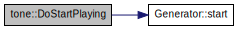
\includegraphics[width=310pt]{classtone_aab27a99690337d475f6be5188798c732_cgraph}
\end{center}
\end{figure}


\hypertarget{classtone_a6f02a174da735dc0947ac4bf151d9012}{\index{tone@{tone}!Get\-Format@{Get\-Format}}
\index{Get\-Format@{Get\-Format}!tone@{tone}}
\subsubsection[{Get\-Format}]{\setlength{\rightskip}{0pt plus 5cm}Q\-Audio\-Format tone\-::\-Get\-Format (
\begin{DoxyParamCaption}
{}
\end{DoxyParamCaption}
)}}\label{classtone_a6f02a174da735dc0947ac4bf151d9012}
\hypertarget{classtone_a07ecdcbc212bfa5a48db8c4e61edb94d}{\index{tone@{tone}!On\-Volume\-Changed@{On\-Volume\-Changed}}
\index{On\-Volume\-Changed@{On\-Volume\-Changed}!tone@{tone}}
\subsubsection[{On\-Volume\-Changed}]{\setlength{\rightskip}{0pt plus 5cm}void tone\-::\-On\-Volume\-Changed (
\begin{DoxyParamCaption}
\item[{int}]{value}
\end{DoxyParamCaption}
)\hspace{0.3cm}{\ttfamily [slot]}}}\label{classtone_a07ecdcbc212bfa5a48db8c4e61edb94d}
\hypertarget{classtone_ad06ca335937de129036a7e79a283f3dd}{\index{tone@{tone}!Pause@{Pause}}
\index{Pause@{Pause}!tone@{tone}}
\subsubsection[{Pause}]{\setlength{\rightskip}{0pt plus 5cm}void tone\-::\-Pause (
\begin{DoxyParamCaption}
{}
\end{DoxyParamCaption}
)}}\label{classtone_ad06ca335937de129036a7e79a283f3dd}
\hypertarget{classtone_ab7c8d92a1041eefbd592f6388c288dc5}{\index{tone@{tone}!Play@{Play}}
\index{Play@{Play}!tone@{tone}}
\subsubsection[{Play}]{\setlength{\rightskip}{0pt plus 5cm}void tone\-::\-Play (
\begin{DoxyParamCaption}
{}
\end{DoxyParamCaption}
)}}\label{classtone_ab7c8d92a1041eefbd592f6388c288dc5}
\hypertarget{classtone_a622c2c46b44e8325f2961c5b60a1c5af}{\index{tone@{tone}!Process@{Process}}
\index{Process@{Process}!tone@{tone}}
\subsubsection[{Process}]{\setlength{\rightskip}{0pt plus 5cm}void tone\-::\-Process (
\begin{DoxyParamCaption}
{}
\end{DoxyParamCaption}
)\hspace{0.3cm}{\ttfamily [slot]}}}\label{classtone_a622c2c46b44e8325f2961c5b60a1c5af}
\hypertarget{classtone_a989956fe95107f983464d2ac01b19211}{\index{tone@{tone}!Set\-Frequency@{Set\-Frequency}}
\index{Set\-Frequency@{Set\-Frequency}!tone@{tone}}
\subsubsection[{Set\-Frequency}]{\setlength{\rightskip}{0pt plus 5cm}void tone\-::\-Set\-Frequency (
\begin{DoxyParamCaption}
\item[{qreal}]{value}
\end{DoxyParamCaption}
)}}\label{classtone_a989956fe95107f983464d2ac01b19211}


Here is the call graph for this function\-:\nopagebreak
\begin{figure}[H]
\begin{center}
\leavevmode
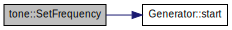
\includegraphics[width=304pt]{classtone_a989956fe95107f983464d2ac01b19211_cgraph}
\end{center}
\end{figure}


\hypertarget{classtone_a241f1871559d339fbdec300dd20da887}{\index{tone@{tone}!Set\-Generator@{Set\-Generator}}
\index{Set\-Generator@{Set\-Generator}!tone@{tone}}
\subsubsection[{Set\-Generator}]{\setlength{\rightskip}{0pt plus 5cm}void tone\-::\-Set\-Generator (
\begin{DoxyParamCaption}
\item[{{\bf Generator} $\ast$}]{gen}
\end{DoxyParamCaption}
)}}\label{classtone_a241f1871559d339fbdec300dd20da887}


Here is the call graph for this function\-:\nopagebreak
\begin{figure}[H]
\begin{center}
\leavevmode
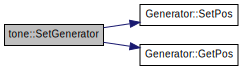
\includegraphics[width=314pt]{classtone_a241f1871559d339fbdec300dd20da887_cgraph}
\end{center}
\end{figure}




\subsection{Member Data Documentation}
\hypertarget{classtone_a8d4a0b1f0f2a3b05fcd580d29e6c7feb}{\index{tone@{tone}!m\-\_\-audio\-Output@{m\-\_\-audio\-Output}}
\index{m\-\_\-audio\-Output@{m\-\_\-audio\-Output}!tone@{tone}}
\subsubsection[{m\-\_\-audio\-Output}]{\setlength{\rightskip}{0pt plus 5cm}Q\-Audio\-Output$\ast$ tone\-::m\-\_\-audio\-Output\hspace{0.3cm}{\ttfamily [protected]}}}\label{classtone_a8d4a0b1f0f2a3b05fcd580d29e6c7feb}
\hypertarget{classtone_a9f2508fefb9803b27bb08276369e2036}{\index{tone@{tone}!m\-\_\-buffer@{m\-\_\-buffer}}
\index{m\-\_\-buffer@{m\-\_\-buffer}!tone@{tone}}
\subsubsection[{m\-\_\-buffer}]{\setlength{\rightskip}{0pt plus 5cm}Q\-Byte\-Array tone\-::m\-\_\-buffer\hspace{0.3cm}{\ttfamily [protected]}}}\label{classtone_a9f2508fefb9803b27bb08276369e2036}
\hypertarget{classtone_ab3c3b5206828b0629a37174ba3b098b1}{\index{tone@{tone}!m\-\_\-device@{m\-\_\-device}}
\index{m\-\_\-device@{m\-\_\-device}!tone@{tone}}
\subsubsection[{m\-\_\-device}]{\setlength{\rightskip}{0pt plus 5cm}Q\-Audio\-Device\-Info tone\-::m\-\_\-device\hspace{0.3cm}{\ttfamily [protected]}}}\label{classtone_ab3c3b5206828b0629a37174ba3b098b1}
\hypertarget{classtone_a556b7109c6895b2c5a3d011145a80952}{\index{tone@{tone}!m\-\_\-format@{m\-\_\-format}}
\index{m\-\_\-format@{m\-\_\-format}!tone@{tone}}
\subsubsection[{m\-\_\-format}]{\setlength{\rightskip}{0pt plus 5cm}Q\-Audio\-Format tone\-::m\-\_\-format\hspace{0.3cm}{\ttfamily [protected]}}}\label{classtone_a556b7109c6895b2c5a3d011145a80952}
\hypertarget{classtone_aa49c08b076903abdbf974444a0efa2b7}{\index{tone@{tone}!m\-\_\-generator@{m\-\_\-generator}}
\index{m\-\_\-generator@{m\-\_\-generator}!tone@{tone}}
\subsubsection[{m\-\_\-generator}]{\setlength{\rightskip}{0pt plus 5cm}{\bf Generator}$\ast$ tone\-::m\-\_\-generator}}\label{classtone_aa49c08b076903abdbf974444a0efa2b7}
\hypertarget{classtone_a97ac901b1b1e269ee5eb719e667485d3}{\index{tone@{tone}!m\-\_\-output@{m\-\_\-output}}
\index{m\-\_\-output@{m\-\_\-output}!tone@{tone}}
\subsubsection[{m\-\_\-output}]{\setlength{\rightskip}{0pt plus 5cm}Q\-I\-O\-Device$\ast$ tone\-::m\-\_\-output\hspace{0.3cm}{\ttfamily [protected]}}}\label{classtone_a97ac901b1b1e269ee5eb719e667485d3}


The documentation for this class was generated from the following files\-:\begin{DoxyCompactItemize}
\item 
Network-\/\-Music/\hyperlink{tone_8h}{tone.\-h}\item 
Network-\/\-Music/\hyperlink{tone_8cpp}{tone.\-cpp}\end{DoxyCompactItemize}

\hypertarget{class_tone_manager}{\section{Tone\-Manager Class Reference}
\label{class_tone_manager}\index{Tone\-Manager@{Tone\-Manager}}
}


{\ttfamily \#include $<$tonemanager.\-h$>$}

\subsection*{Public Slots}
\begin{DoxyCompactItemize}
\item 
void \hyperlink{class_tone_manager_a4491c3853b267e69d839e5d07db6c65f}{S\-L\-O\-T\-\_\-\-Number\-Of\-Tones\-Changed} (int new\-Number\-Of\-Tones)
\item 
void \hyperlink{class_tone_manager_af3235b97bd5eb323707df906c2057194}{S\-L\-O\-T\-\_\-\-Volume\-Changed} (int new\-Volume)
\item 
void \hyperlink{class_tone_manager_a012e94dca7cfd276a5d84d79c9d8564d}{S\-L\-O\-T\-\_\-\-Set\-Frequency} (int frequency, int often)
\item 
void \hyperlink{class_tone_manager_a9b7baa7bd7d8b3a25dc37c700439dfff}{S\-L\-O\-T\-\_\-\-Set\-Base\-Frequency} (int base\-Frequency)
\item 
void \hyperlink{class_tone_manager_a2de4f382875c53549d203e37c03a1b5c}{S\-L\-O\-T\-\_\-\-Initialize\-Tones} ()
\end{DoxyCompactItemize}
\subsection*{Signals}
\begin{DoxyCompactItemize}
\item 
void \hyperlink{class_tone_manager_a350057c72bfef92eafd78fcf663a4780}{Set\-\_\-\-Volume} (int)
\item 
void \hyperlink{class_tone_manager_adef20253e76dd81cb8b730a04a4c611d}{Resume\-\_\-\-Audio} ()
\item 
void \hyperlink{class_tone_manager_a1585c35147c628bffcca0683d87e9275}{Pause\-\_\-\-Audio} ()
\item 
void \hyperlink{class_tone_manager_a9c6253effbaab4dca2b087bc4ab88598}{Start\-\_\-\-Audio} ()
\end{DoxyCompactItemize}
\subsection*{Public Member Functions}
\begin{DoxyCompactItemize}
\item 
\hyperlink{class_tone_manager_a8638f3e1194ff8745c867e32b4da6c9b}{Tone\-Manager} ()
\item 
\hyperlink{class_tone_manager_adce76ae3f2ae844fbed2c56a3100a3c9}{Tone\-Manager} (int Base\-Number\-Of\-Tones)
\item 
\hyperlink{class_tone_manager_ae244662cb3d420d41e3f0a178b5cdfdf}{$\sim$\-Tone\-Manager} ()
\end{DoxyCompactItemize}
\subsection*{Protected Member Functions}
\begin{DoxyCompactItemize}
\item 
\hyperlink{struct_tone_object}{Tone\-Object} $\ast$ \hyperlink{class_tone_manager_a5145a5a45c5b673c0301550285a04b61}{Add\-Tone} (int i)
\end{DoxyCompactItemize}
\subsection*{Protected Attributes}
\begin{DoxyCompactItemize}
\item 
int \hyperlink{class_tone_manager_ab5c9a0920466d82f885472f6b00d8874}{number\-Of\-Tones}
\item 
int \hyperlink{class_tone_manager_af00d6b668bdb26c6f2945495f6ef65c5}{current\-Tone}
\item 
int \hyperlink{class_tone_manager_a1a3f2a72be83f2e28766f72bc5b10222}{current\-Uncommon\-Tone}
\item 
int \hyperlink{class_tone_manager_a13b80ecf3d51ae30210fbe99c5bb2863}{tone\-Base\-Frequency}
\item 
Q\-Audio\-Format \hyperlink{class_tone_manager_ac3ffa52adeeacd270c60845052acf277}{m\-\_\-format}
\item 
Q\-Hash$<$ int, Q\-Byte\-Array $\ast$ $>$ \hyperlink{class_tone_manager_a7f2598af2eb46a6a9ee99bad59aa6db8}{tone\-Buffers}
\item 
Q\-List$<$ \hyperlink{struct_tone_object}{Tone\-Object} $\ast$ $>$ \hyperlink{class_tone_manager_a237856f80ab73ae89e32f59f6962ed41}{Tones}
\end{DoxyCompactItemize}


\subsection{Detailed Description}
Class that acts as the controller to the tones 

\subsection{Constructor \& Destructor Documentation}
\hypertarget{class_tone_manager_a8638f3e1194ff8745c867e32b4da6c9b}{\index{Tone\-Manager@{Tone\-Manager}!Tone\-Manager@{Tone\-Manager}}
\index{Tone\-Manager@{Tone\-Manager}!ToneManager@{Tone\-Manager}}
\subsubsection[{Tone\-Manager}]{\setlength{\rightskip}{0pt plus 5cm}Tone\-Manager\-::\-Tone\-Manager (
\begin{DoxyParamCaption}
{}
\end{DoxyParamCaption}
)}}\label{class_tone_manager_a8638f3e1194ff8745c867e32b4da6c9b}
\hypertarget{class_tone_manager_adce76ae3f2ae844fbed2c56a3100a3c9}{\index{Tone\-Manager@{Tone\-Manager}!Tone\-Manager@{Tone\-Manager}}
\index{Tone\-Manager@{Tone\-Manager}!ToneManager@{Tone\-Manager}}
\subsubsection[{Tone\-Manager}]{\setlength{\rightskip}{0pt plus 5cm}Tone\-Manager\-::\-Tone\-Manager (
\begin{DoxyParamCaption}
\item[{int}]{Base\-Number\-Of\-Tones = {\ttfamily {\bf T\-O\-N\-E\-\_\-\-C\-O\-U\-N\-T}}}
\end{DoxyParamCaption}
)}}\label{class_tone_manager_adce76ae3f2ae844fbed2c56a3100a3c9}
\hypertarget{class_tone_manager_ae244662cb3d420d41e3f0a178b5cdfdf}{\index{Tone\-Manager@{Tone\-Manager}!$\sim$\-Tone\-Manager@{$\sim$\-Tone\-Manager}}
\index{$\sim$\-Tone\-Manager@{$\sim$\-Tone\-Manager}!ToneManager@{Tone\-Manager}}
\subsubsection[{$\sim$\-Tone\-Manager}]{\setlength{\rightskip}{0pt plus 5cm}Tone\-Manager\-::$\sim$\-Tone\-Manager (
\begin{DoxyParamCaption}
{}
\end{DoxyParamCaption}
)}}\label{class_tone_manager_ae244662cb3d420d41e3f0a178b5cdfdf}


\subsection{Member Function Documentation}
\hypertarget{class_tone_manager_a5145a5a45c5b673c0301550285a04b61}{\index{Tone\-Manager@{Tone\-Manager}!Add\-Tone@{Add\-Tone}}
\index{Add\-Tone@{Add\-Tone}!ToneManager@{Tone\-Manager}}
\subsubsection[{Add\-Tone}]{\setlength{\rightskip}{0pt plus 5cm}{\bf Tone\-Object} $\ast$ Tone\-Manager\-::\-Add\-Tone (
\begin{DoxyParamCaption}
\item[{int}]{i}
\end{DoxyParamCaption}
)\hspace{0.3cm}{\ttfamily [protected]}}}\label{class_tone_manager_a5145a5a45c5b673c0301550285a04b61}


Here is the caller graph for this function\-:
\nopagebreak
\begin{figure}[H]
\begin{center}
\leavevmode
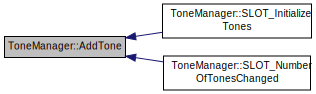
\includegraphics[width=350pt]{class_tone_manager_a5145a5a45c5b673c0301550285a04b61_icgraph}
\end{center}
\end{figure}


\hypertarget{class_tone_manager_a1585c35147c628bffcca0683d87e9275}{\index{Tone\-Manager@{Tone\-Manager}!Pause\-\_\-\-Audio@{Pause\-\_\-\-Audio}}
\index{Pause\-\_\-\-Audio@{Pause\-\_\-\-Audio}!ToneManager@{Tone\-Manager}}
\subsubsection[{Pause\-\_\-\-Audio}]{\setlength{\rightskip}{0pt plus 5cm}void Tone\-Manager\-::\-Pause\-\_\-\-Audio (
\begin{DoxyParamCaption}
{}
\end{DoxyParamCaption}
)\hspace{0.3cm}{\ttfamily [signal]}}}\label{class_tone_manager_a1585c35147c628bffcca0683d87e9275}


Here is the caller graph for this function\-:
\nopagebreak
\begin{figure}[H]
\begin{center}
\leavevmode
\includegraphics[width=350pt]{class_tone_manager_a1585c35147c628bffcca0683d87e9275_icgraph}
\end{center}
\end{figure}


\hypertarget{class_tone_manager_adef20253e76dd81cb8b730a04a4c611d}{\index{Tone\-Manager@{Tone\-Manager}!Resume\-\_\-\-Audio@{Resume\-\_\-\-Audio}}
\index{Resume\-\_\-\-Audio@{Resume\-\_\-\-Audio}!ToneManager@{Tone\-Manager}}
\subsubsection[{Resume\-\_\-\-Audio}]{\setlength{\rightskip}{0pt plus 5cm}void Tone\-Manager\-::\-Resume\-\_\-\-Audio (
\begin{DoxyParamCaption}
{}
\end{DoxyParamCaption}
)\hspace{0.3cm}{\ttfamily [signal]}}}\label{class_tone_manager_adef20253e76dd81cb8b730a04a4c611d}


Here is the caller graph for this function\-:
\nopagebreak
\begin{figure}[H]
\begin{center}
\leavevmode
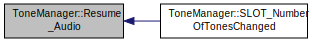
\includegraphics[width=350pt]{class_tone_manager_adef20253e76dd81cb8b730a04a4c611d_icgraph}
\end{center}
\end{figure}


\hypertarget{class_tone_manager_a350057c72bfef92eafd78fcf663a4780}{\index{Tone\-Manager@{Tone\-Manager}!Set\-\_\-\-Volume@{Set\-\_\-\-Volume}}
\index{Set\-\_\-\-Volume@{Set\-\_\-\-Volume}!ToneManager@{Tone\-Manager}}
\subsubsection[{Set\-\_\-\-Volume}]{\setlength{\rightskip}{0pt plus 5cm}void Tone\-Manager\-::\-Set\-\_\-\-Volume (
\begin{DoxyParamCaption}
\item[{int}]{}
\end{DoxyParamCaption}
)\hspace{0.3cm}{\ttfamily [signal]}}}\label{class_tone_manager_a350057c72bfef92eafd78fcf663a4780}


Here is the caller graph for this function\-:
\nopagebreak
\begin{figure}[H]
\begin{center}
\leavevmode
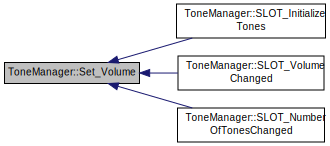
\includegraphics[width=350pt]{class_tone_manager_a350057c72bfef92eafd78fcf663a4780_icgraph}
\end{center}
\end{figure}


\hypertarget{class_tone_manager_a2de4f382875c53549d203e37c03a1b5c}{\index{Tone\-Manager@{Tone\-Manager}!S\-L\-O\-T\-\_\-\-Initialize\-Tones@{S\-L\-O\-T\-\_\-\-Initialize\-Tones}}
\index{S\-L\-O\-T\-\_\-\-Initialize\-Tones@{S\-L\-O\-T\-\_\-\-Initialize\-Tones}!ToneManager@{Tone\-Manager}}
\subsubsection[{S\-L\-O\-T\-\_\-\-Initialize\-Tones}]{\setlength{\rightskip}{0pt plus 5cm}void Tone\-Manager\-::\-S\-L\-O\-T\-\_\-\-Initialize\-Tones (
\begin{DoxyParamCaption}
{}
\end{DoxyParamCaption}
)\hspace{0.3cm}{\ttfamily [slot]}}}\label{class_tone_manager_a2de4f382875c53549d203e37c03a1b5c}


Here is the call graph for this function\-:
\nopagebreak
\begin{figure}[H]
\begin{center}
\leavevmode
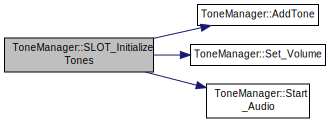
\includegraphics[width=350pt]{class_tone_manager_a2de4f382875c53549d203e37c03a1b5c_cgraph}
\end{center}
\end{figure}


\hypertarget{class_tone_manager_a4491c3853b267e69d839e5d07db6c65f}{\index{Tone\-Manager@{Tone\-Manager}!S\-L\-O\-T\-\_\-\-Number\-Of\-Tones\-Changed@{S\-L\-O\-T\-\_\-\-Number\-Of\-Tones\-Changed}}
\index{S\-L\-O\-T\-\_\-\-Number\-Of\-Tones\-Changed@{S\-L\-O\-T\-\_\-\-Number\-Of\-Tones\-Changed}!ToneManager@{Tone\-Manager}}
\subsubsection[{S\-L\-O\-T\-\_\-\-Number\-Of\-Tones\-Changed}]{\setlength{\rightskip}{0pt plus 5cm}void Tone\-Manager\-::\-S\-L\-O\-T\-\_\-\-Number\-Of\-Tones\-Changed (
\begin{DoxyParamCaption}
\item[{int}]{new\-Number\-Of\-Tones}
\end{DoxyParamCaption}
)\hspace{0.3cm}{\ttfamily [slot]}}}\label{class_tone_manager_a4491c3853b267e69d839e5d07db6c65f}
Very clunky 

Here is the call graph for this function\-:
\nopagebreak
\begin{figure}[H]
\begin{center}
\leavevmode
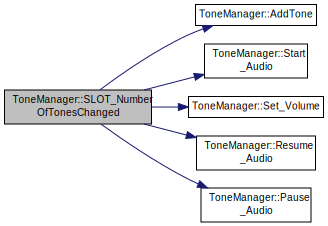
\includegraphics[width=350pt]{class_tone_manager_a4491c3853b267e69d839e5d07db6c65f_cgraph}
\end{center}
\end{figure}


\hypertarget{class_tone_manager_a9b7baa7bd7d8b3a25dc37c700439dfff}{\index{Tone\-Manager@{Tone\-Manager}!S\-L\-O\-T\-\_\-\-Set\-Base\-Frequency@{S\-L\-O\-T\-\_\-\-Set\-Base\-Frequency}}
\index{S\-L\-O\-T\-\_\-\-Set\-Base\-Frequency@{S\-L\-O\-T\-\_\-\-Set\-Base\-Frequency}!ToneManager@{Tone\-Manager}}
\subsubsection[{S\-L\-O\-T\-\_\-\-Set\-Base\-Frequency}]{\setlength{\rightskip}{0pt plus 5cm}void Tone\-Manager\-::\-S\-L\-O\-T\-\_\-\-Set\-Base\-Frequency (
\begin{DoxyParamCaption}
\item[{int}]{base\-Frequency}
\end{DoxyParamCaption}
)\hspace{0.3cm}{\ttfamily [slot]}}}\label{class_tone_manager_a9b7baa7bd7d8b3a25dc37c700439dfff}
\hypertarget{class_tone_manager_a012e94dca7cfd276a5d84d79c9d8564d}{\index{Tone\-Manager@{Tone\-Manager}!S\-L\-O\-T\-\_\-\-Set\-Frequency@{S\-L\-O\-T\-\_\-\-Set\-Frequency}}
\index{S\-L\-O\-T\-\_\-\-Set\-Frequency@{S\-L\-O\-T\-\_\-\-Set\-Frequency}!ToneManager@{Tone\-Manager}}
\subsubsection[{S\-L\-O\-T\-\_\-\-Set\-Frequency}]{\setlength{\rightskip}{0pt plus 5cm}void Tone\-Manager\-::\-S\-L\-O\-T\-\_\-\-Set\-Frequency (
\begin{DoxyParamCaption}
\item[{int}]{frequency, }
\item[{int}]{often}
\end{DoxyParamCaption}
)\hspace{0.3cm}{\ttfamily [slot]}}}\label{class_tone_manager_a012e94dca7cfd276a5d84d79c9d8564d}
\begin{DoxyAttention}{Attention}
modify the frequency for \char`\"{}niceness\char`\"{} 
\end{DoxyAttention}


Here is the call graph for this function\-:
\nopagebreak
\begin{figure}[H]
\begin{center}
\leavevmode
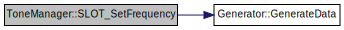
\includegraphics[width=350pt]{class_tone_manager_a012e94dca7cfd276a5d84d79c9d8564d_cgraph}
\end{center}
\end{figure}


\hypertarget{class_tone_manager_af3235b97bd5eb323707df906c2057194}{\index{Tone\-Manager@{Tone\-Manager}!S\-L\-O\-T\-\_\-\-Volume\-Changed@{S\-L\-O\-T\-\_\-\-Volume\-Changed}}
\index{S\-L\-O\-T\-\_\-\-Volume\-Changed@{S\-L\-O\-T\-\_\-\-Volume\-Changed}!ToneManager@{Tone\-Manager}}
\subsubsection[{S\-L\-O\-T\-\_\-\-Volume\-Changed}]{\setlength{\rightskip}{0pt plus 5cm}void Tone\-Manager\-::\-S\-L\-O\-T\-\_\-\-Volume\-Changed (
\begin{DoxyParamCaption}
\item[{int}]{new\-Volume}
\end{DoxyParamCaption}
)\hspace{0.3cm}{\ttfamily [slot]}}}\label{class_tone_manager_af3235b97bd5eb323707df906c2057194}


Here is the call graph for this function\-:
\nopagebreak
\begin{figure}[H]
\begin{center}
\leavevmode
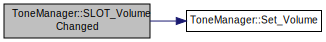
\includegraphics[width=350pt]{class_tone_manager_af3235b97bd5eb323707df906c2057194_cgraph}
\end{center}
\end{figure}


\hypertarget{class_tone_manager_a9c6253effbaab4dca2b087bc4ab88598}{\index{Tone\-Manager@{Tone\-Manager}!Start\-\_\-\-Audio@{Start\-\_\-\-Audio}}
\index{Start\-\_\-\-Audio@{Start\-\_\-\-Audio}!ToneManager@{Tone\-Manager}}
\subsubsection[{Start\-\_\-\-Audio}]{\setlength{\rightskip}{0pt plus 5cm}void Tone\-Manager\-::\-Start\-\_\-\-Audio (
\begin{DoxyParamCaption}
{}
\end{DoxyParamCaption}
)\hspace{0.3cm}{\ttfamily [signal]}}}\label{class_tone_manager_a9c6253effbaab4dca2b087bc4ab88598}


Here is the caller graph for this function\-:
\nopagebreak
\begin{figure}[H]
\begin{center}
\leavevmode
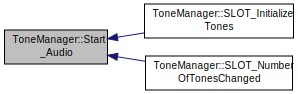
\includegraphics[width=350pt]{class_tone_manager_a9c6253effbaab4dca2b087bc4ab88598_icgraph}
\end{center}
\end{figure}




\subsection{Member Data Documentation}
\hypertarget{class_tone_manager_af00d6b668bdb26c6f2945495f6ef65c5}{\index{Tone\-Manager@{Tone\-Manager}!current\-Tone@{current\-Tone}}
\index{current\-Tone@{current\-Tone}!ToneManager@{Tone\-Manager}}
\subsubsection[{current\-Tone}]{\setlength{\rightskip}{0pt plus 5cm}int Tone\-Manager\-::current\-Tone\hspace{0.3cm}{\ttfamily [protected]}}}\label{class_tone_manager_af00d6b668bdb26c6f2945495f6ef65c5}
\hypertarget{class_tone_manager_a1a3f2a72be83f2e28766f72bc5b10222}{\index{Tone\-Manager@{Tone\-Manager}!current\-Uncommon\-Tone@{current\-Uncommon\-Tone}}
\index{current\-Uncommon\-Tone@{current\-Uncommon\-Tone}!ToneManager@{Tone\-Manager}}
\subsubsection[{current\-Uncommon\-Tone}]{\setlength{\rightskip}{0pt plus 5cm}int Tone\-Manager\-::current\-Uncommon\-Tone\hspace{0.3cm}{\ttfamily [protected]}}}\label{class_tone_manager_a1a3f2a72be83f2e28766f72bc5b10222}
\hypertarget{class_tone_manager_ac3ffa52adeeacd270c60845052acf277}{\index{Tone\-Manager@{Tone\-Manager}!m\-\_\-format@{m\-\_\-format}}
\index{m\-\_\-format@{m\-\_\-format}!ToneManager@{Tone\-Manager}}
\subsubsection[{m\-\_\-format}]{\setlength{\rightskip}{0pt plus 5cm}Q\-Audio\-Format Tone\-Manager\-::m\-\_\-format\hspace{0.3cm}{\ttfamily [protected]}}}\label{class_tone_manager_ac3ffa52adeeacd270c60845052acf277}
\hypertarget{class_tone_manager_ab5c9a0920466d82f885472f6b00d8874}{\index{Tone\-Manager@{Tone\-Manager}!number\-Of\-Tones@{number\-Of\-Tones}}
\index{number\-Of\-Tones@{number\-Of\-Tones}!ToneManager@{Tone\-Manager}}
\subsubsection[{number\-Of\-Tones}]{\setlength{\rightskip}{0pt plus 5cm}int Tone\-Manager\-::number\-Of\-Tones\hspace{0.3cm}{\ttfamily [protected]}}}\label{class_tone_manager_ab5c9a0920466d82f885472f6b00d8874}
\hypertarget{class_tone_manager_a13b80ecf3d51ae30210fbe99c5bb2863}{\index{Tone\-Manager@{Tone\-Manager}!tone\-Base\-Frequency@{tone\-Base\-Frequency}}
\index{tone\-Base\-Frequency@{tone\-Base\-Frequency}!ToneManager@{Tone\-Manager}}
\subsubsection[{tone\-Base\-Frequency}]{\setlength{\rightskip}{0pt plus 5cm}int Tone\-Manager\-::tone\-Base\-Frequency\hspace{0.3cm}{\ttfamily [protected]}}}\label{class_tone_manager_a13b80ecf3d51ae30210fbe99c5bb2863}
\hypertarget{class_tone_manager_a7f2598af2eb46a6a9ee99bad59aa6db8}{\index{Tone\-Manager@{Tone\-Manager}!tone\-Buffers@{tone\-Buffers}}
\index{tone\-Buffers@{tone\-Buffers}!ToneManager@{Tone\-Manager}}
\subsubsection[{tone\-Buffers}]{\setlength{\rightskip}{0pt plus 5cm}Q\-Hash$<$int, Q\-Byte\-Array$\ast$$>$ Tone\-Manager\-::tone\-Buffers\hspace{0.3cm}{\ttfamily [protected]}}}\label{class_tone_manager_a7f2598af2eb46a6a9ee99bad59aa6db8}
\hypertarget{class_tone_manager_a237856f80ab73ae89e32f59f6962ed41}{\index{Tone\-Manager@{Tone\-Manager}!Tones@{Tones}}
\index{Tones@{Tones}!ToneManager@{Tone\-Manager}}
\subsubsection[{Tones}]{\setlength{\rightskip}{0pt plus 5cm}Q\-List$<${\bf Tone\-Object}$\ast$$>$ Tone\-Manager\-::\-Tones\hspace{0.3cm}{\ttfamily [protected]}}}\label{class_tone_manager_a237856f80ab73ae89e32f59f6962ed41}


The documentation for this class was generated from the following files\-:\begin{DoxyCompactItemize}
\item 
Network-\/\-Music/\hyperlink{tonemanager_8h}{tonemanager.\-h}\item 
Network-\/\-Music/\hyperlink{tonemanager_8cpp}{tonemanager.\-cpp}\end{DoxyCompactItemize}

\hypertarget{struct_tone_object}{\section{Tone\-Object Struct Reference}
\label{struct_tone_object}\index{Tone\-Object@{Tone\-Object}}
}


{\ttfamily \#include $<$tonemanager.\-h$>$}



Collaboration diagram for Tone\-Object\-:
\nopagebreak
\begin{figure}[H]
\begin{center}
\leavevmode
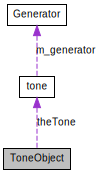
\includegraphics[width=171pt]{struct_tone_object__coll__graph}
\end{center}
\end{figure}
\subsection*{Public Attributes}
\begin{DoxyCompactItemize}
\item 
\hyperlink{classtone}{tone} $\ast$ \hyperlink{struct_tone_object_a47610a83de0887b5c8e5d8e009312958}{the\-Tone}
\item 
Q\-Thread $\ast$ \hyperlink{struct_tone_object_abeb12728a40883a44c0440db7dbb1732}{the\-Thread}
\end{DoxyCompactItemize}


\subsection{Member Data Documentation}
\hypertarget{struct_tone_object_abeb12728a40883a44c0440db7dbb1732}{\index{Tone\-Object@{Tone\-Object}!the\-Thread@{the\-Thread}}
\index{the\-Thread@{the\-Thread}!ToneObject@{Tone\-Object}}
\subsubsection[{the\-Thread}]{\setlength{\rightskip}{0pt plus 5cm}Q\-Thread$\ast$ Tone\-Object\-::the\-Thread}}\label{struct_tone_object_abeb12728a40883a44c0440db7dbb1732}
\hypertarget{struct_tone_object_a47610a83de0887b5c8e5d8e009312958}{\index{Tone\-Object@{Tone\-Object}!the\-Tone@{the\-Tone}}
\index{the\-Tone@{the\-Tone}!ToneObject@{Tone\-Object}}
\subsubsection[{the\-Tone}]{\setlength{\rightskip}{0pt plus 5cm}{\bf tone}$\ast$ Tone\-Object\-::the\-Tone}}\label{struct_tone_object_a47610a83de0887b5c8e5d8e009312958}


The documentation for this struct was generated from the following file\-:\begin{DoxyCompactItemize}
\item 
Network-\/\-Music/\hyperlink{tonemanager_8h}{tonemanager.\-h}\end{DoxyCompactItemize}

\chapter{File Documentation}
\hypertarget{audiograph_8cpp}{\section{Network-\/\-Music/audiograph.cpp File Reference}
\label{audiograph_8cpp}\index{Network-\/\-Music/audiograph.\-cpp@{Network-\/\-Music/audiograph.\-cpp}}
}
{\ttfamily \#include \char`\"{}audiograph.\-h\char`\"{}}\\*
Include dependency graph for audiograph.\-cpp\-:
\nopagebreak
\begin{figure}[H]
\begin{center}
\leavevmode
\includegraphics[width=350pt]{audiograph_8cpp__incl}
\end{center}
\end{figure}
\subsection*{Macros}
\begin{DoxyCompactItemize}
\item 
\#define \hyperlink{audiograph_8cpp_a79f68dadd4ade072fc7121cfe2c40b30}{T\-I\-M\-E\-R\-\_\-\-T\-I\-C\-K}~(1000)
\item 
\#define \hyperlink{audiograph_8cpp_a933875ad2e948ac7326bac2341740cf0}{T\-I\-M\-E\-\_\-\-R\-A\-N\-G\-E}~(30)
\end{DoxyCompactItemize}
\subsection*{Variables}
\begin{DoxyCompactItemize}
\item 
const int \hyperlink{audiograph_8cpp_a40ecd6c75beb060288e312379ffd1d44}{number\-Of\-Items} = 3600
\item 
const float \hyperlink{audiograph_8cpp_a226f60633113fe6fe6e37d6c05ec2789}{curve\-Divider} = 3.\-0f
\item 
const int \hyperlink{audiograph_8cpp_ac46566db1800e80494a56aed488d6dfa}{lower\-Number\-Of\-Items} = 900
\item 
const float \hyperlink{audiograph_8cpp_ae34bfaae4dcb3c0caf5106c60e501b44}{lower\-Curve\-Divider} = 0.\-75f
\end{DoxyCompactItemize}


\subsection{Macro Definition Documentation}
\hypertarget{audiograph_8cpp_a933875ad2e948ac7326bac2341740cf0}{\index{audiograph.\-cpp@{audiograph.\-cpp}!T\-I\-M\-E\-\_\-\-R\-A\-N\-G\-E@{T\-I\-M\-E\-\_\-\-R\-A\-N\-G\-E}}
\index{T\-I\-M\-E\-\_\-\-R\-A\-N\-G\-E@{T\-I\-M\-E\-\_\-\-R\-A\-N\-G\-E}!audiograph.cpp@{audiograph.\-cpp}}
\subsubsection[{T\-I\-M\-E\-\_\-\-R\-A\-N\-G\-E}]{\setlength{\rightskip}{0pt plus 5cm}\#define T\-I\-M\-E\-\_\-\-R\-A\-N\-G\-E~(30)}}\label{audiograph_8cpp_a933875ad2e948ac7326bac2341740cf0}
\hypertarget{audiograph_8cpp_a79f68dadd4ade072fc7121cfe2c40b30}{\index{audiograph.\-cpp@{audiograph.\-cpp}!T\-I\-M\-E\-R\-\_\-\-T\-I\-C\-K@{T\-I\-M\-E\-R\-\_\-\-T\-I\-C\-K}}
\index{T\-I\-M\-E\-R\-\_\-\-T\-I\-C\-K@{T\-I\-M\-E\-R\-\_\-\-T\-I\-C\-K}!audiograph.cpp@{audiograph.\-cpp}}
\subsubsection[{T\-I\-M\-E\-R\-\_\-\-T\-I\-C\-K}]{\setlength{\rightskip}{0pt plus 5cm}\#define T\-I\-M\-E\-R\-\_\-\-T\-I\-C\-K~(1000)}}\label{audiograph_8cpp_a79f68dadd4ade072fc7121cfe2c40b30}


\subsection{Variable Documentation}
\hypertarget{audiograph_8cpp_a226f60633113fe6fe6e37d6c05ec2789}{\index{audiograph.\-cpp@{audiograph.\-cpp}!curve\-Divider@{curve\-Divider}}
\index{curve\-Divider@{curve\-Divider}!audiograph.cpp@{audiograph.\-cpp}}
\subsubsection[{curve\-Divider}]{\setlength{\rightskip}{0pt plus 5cm}const float curve\-Divider = 3.\-0f}}\label{audiograph_8cpp_a226f60633113fe6fe6e37d6c05ec2789}
\hypertarget{audiograph_8cpp_ae34bfaae4dcb3c0caf5106c60e501b44}{\index{audiograph.\-cpp@{audiograph.\-cpp}!lower\-Curve\-Divider@{lower\-Curve\-Divider}}
\index{lower\-Curve\-Divider@{lower\-Curve\-Divider}!audiograph.cpp@{audiograph.\-cpp}}
\subsubsection[{lower\-Curve\-Divider}]{\setlength{\rightskip}{0pt plus 5cm}const float lower\-Curve\-Divider = 0.\-75f}}\label{audiograph_8cpp_ae34bfaae4dcb3c0caf5106c60e501b44}
\hypertarget{audiograph_8cpp_ac46566db1800e80494a56aed488d6dfa}{\index{audiograph.\-cpp@{audiograph.\-cpp}!lower\-Number\-Of\-Items@{lower\-Number\-Of\-Items}}
\index{lower\-Number\-Of\-Items@{lower\-Number\-Of\-Items}!audiograph.cpp@{audiograph.\-cpp}}
\subsubsection[{lower\-Number\-Of\-Items}]{\setlength{\rightskip}{0pt plus 5cm}const int lower\-Number\-Of\-Items = 900}}\label{audiograph_8cpp_ac46566db1800e80494a56aed488d6dfa}
\hypertarget{audiograph_8cpp_a40ecd6c75beb060288e312379ffd1d44}{\index{audiograph.\-cpp@{audiograph.\-cpp}!number\-Of\-Items@{number\-Of\-Items}}
\index{number\-Of\-Items@{number\-Of\-Items}!audiograph.cpp@{audiograph.\-cpp}}
\subsubsection[{number\-Of\-Items}]{\setlength{\rightskip}{0pt plus 5cm}const int number\-Of\-Items = 3600}}\label{audiograph_8cpp_a40ecd6c75beb060288e312379ffd1d44}

\hypertarget{audiograph_8h}{\section{Network-\/\-Music/audiograph.h File Reference}
\label{audiograph_8h}\index{Network-\/\-Music/audiograph.\-h@{Network-\/\-Music/audiograph.\-h}}
}
{\ttfamily \#include $<$Qt\-Data\-Visualization/q3dscatter.\-h$>$}\\*
{\ttfamily \#include $<$Qt\-Data\-Visualization/qabstract3dseries.\-h$>$}\\*
{\ttfamily \#include $<$Qt\-Gui/\-Q\-Font$>$}\\*
{\ttfamily \#include $<$Qt\-Widgets/\-Q\-Application$>$}\\*
{\ttfamily \#include $<$Qt\-Widgets/\-Q\-Widget$>$}\\*
{\ttfamily \#include $<$Qt\-Widgets/\-Q\-H\-Box\-Layout$>$}\\*
{\ttfamily \#include $<$Qt\-Widgets/\-Q\-V\-Box\-Layout$>$}\\*
{\ttfamily \#include $<$Qt\-Widgets/\-Q\-Push\-Button$>$}\\*
{\ttfamily \#include $<$Qt\-Widgets/\-Q\-Check\-Box$>$}\\*
{\ttfamily \#include $<$Qt\-Widgets/\-Q\-Combo\-Box$>$}\\*
{\ttfamily \#include $<$Qt\-Widgets/\-Q\-Font\-Combo\-Box$>$}\\*
{\ttfamily \#include $<$Qt\-Widgets/\-Q\-Label$>$}\\*
{\ttfamily \#include $<$Qt\-Gui/\-Q\-Screen$>$}\\*
{\ttfamily \#include $<$Qt\-Gui/\-Q\-Font\-Database$>$}\\*
{\ttfamily \#include $<$Q\-Timer$>$}\\*
Include dependency graph for audiograph.\-h\-:
\nopagebreak
\begin{figure}[H]
\begin{center}
\leavevmode
\includegraphics[width=350pt]{audiograph_8h__incl}
\end{center}
\end{figure}
This graph shows which files directly or indirectly include this file\-:
\nopagebreak
\begin{figure}[H]
\begin{center}
\leavevmode
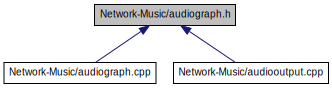
\includegraphics[width=350pt]{audiograph_8h__dep__incl}
\end{center}
\end{figure}
\subsection*{Classes}
\begin{DoxyCompactItemize}
\item 
class \hyperlink{class_audio_graph}{Audio\-Graph}
\end{DoxyCompactItemize}

\hypertarget{audiooutput_8cpp}{\section{Network-\/\-Music/audiooutput.cpp File Reference}
\label{audiooutput_8cpp}\index{Network-\/\-Music/audiooutput.\-cpp@{Network-\/\-Music/audiooutput.\-cpp}}
}
{\ttfamily \#include $<$Q\-Audio\-Device\-Info$>$}\\*
{\ttfamily \#include $<$Q\-Audio\-Output$>$}\\*
{\ttfamily \#include $<$Q\-Debug$>$}\\*
{\ttfamily \#include $<$Q\-V\-Box\-Layout$>$}\\*
{\ttfamily \#include $<$qmath.\-h$>$}\\*
{\ttfamily \#include $<$qendian.\-h$>$}\\*
{\ttfamily \#include $<$Q\-Hash$>$}\\*
{\ttfamily \#include $<$Q\-Thread$>$}\\*
{\ttfamily \#include $<$pcap.\-h$>$}\\*
{\ttfamily \#include \char`\"{}audiooutput.\-h\char`\"{}}\\*
{\ttfamily \#include \char`\"{}tone.\-h\char`\"{}}\\*
{\ttfamily \#include \char`\"{}packetcapturer.\-h\char`\"{}}\\*
{\ttfamily \#include \char`\"{}tonemanager.\-h\char`\"{}}\\*
{\ttfamily \#include \char`\"{}audiograph.\-h\char`\"{}}\\*
Include dependency graph for audiooutput.\-cpp\-:
\nopagebreak
\begin{figure}[H]
\begin{center}
\leavevmode
\includegraphics[width=350pt]{audiooutput_8cpp__incl}
\end{center}
\end{figure}
\subsection*{Macros}
\begin{DoxyCompactItemize}
\item 
\#define \hyperlink{audiooutput_8cpp_a7a18f02620ad721f668eb718157f11e8}{S\-U\-S\-P\-E\-N\-D\-\_\-\-L\-A\-B\-E\-L}~\char`\"{}Suspend playback\char`\"{}
\item 
\#define \hyperlink{audiooutput_8cpp_af266e8e5dfbb807dec167c97f68a3767}{R\-E\-S\-U\-M\-E\-\_\-\-L\-A\-B\-E\-L}~\char`\"{}Resume playback\char`\"{}
\item 
\#define \hyperlink{audiooutput_8cpp_a4ca48866c33da3c81aec1dfd571f2054}{V\-O\-L\-U\-M\-E\-\_\-\-L\-A\-B\-E\-L}~\char`\"{}Volume\-:\char`\"{}
\item 
\#define \hyperlink{audiooutput_8cpp_a1be5b24cec173ec08c04dc6faf91c5da}{T\-O\-N\-E\-\_\-\-M\-A\-X}~(15)
\item 
\#define \hyperlink{audiooutput_8cpp_a3760582a7103aaa001751069d0d1c1f2}{T\-O\-N\-E\-\_\-\-M\-I\-N}~(3)
\item 
\#define \hyperlink{audiooutput_8cpp_a5e6855de8203fe9ae34cf63f68799e98}{T\-O\-N\-E\-\_\-\-C\-O\-U\-N\-T}~(5)
\item 
\#define \hyperlink{audiooutput_8cpp_ad826826fe755da59dcff55bf092c9ed8}{M\-A\-X\-\_\-\-S\-L\-I\-C\-E\-S}~(10)
\end{DoxyCompactItemize}


\subsection{Macro Definition Documentation}
\hypertarget{audiooutput_8cpp_ad826826fe755da59dcff55bf092c9ed8}{\index{audiooutput.\-cpp@{audiooutput.\-cpp}!M\-A\-X\-\_\-\-S\-L\-I\-C\-E\-S@{M\-A\-X\-\_\-\-S\-L\-I\-C\-E\-S}}
\index{M\-A\-X\-\_\-\-S\-L\-I\-C\-E\-S@{M\-A\-X\-\_\-\-S\-L\-I\-C\-E\-S}!audiooutput.cpp@{audiooutput.\-cpp}}
\subsubsection[{M\-A\-X\-\_\-\-S\-L\-I\-C\-E\-S}]{\setlength{\rightskip}{0pt plus 5cm}\#define M\-A\-X\-\_\-\-S\-L\-I\-C\-E\-S~(10)}}\label{audiooutput_8cpp_ad826826fe755da59dcff55bf092c9ed8}
\hypertarget{audiooutput_8cpp_af266e8e5dfbb807dec167c97f68a3767}{\index{audiooutput.\-cpp@{audiooutput.\-cpp}!R\-E\-S\-U\-M\-E\-\_\-\-L\-A\-B\-E\-L@{R\-E\-S\-U\-M\-E\-\_\-\-L\-A\-B\-E\-L}}
\index{R\-E\-S\-U\-M\-E\-\_\-\-L\-A\-B\-E\-L@{R\-E\-S\-U\-M\-E\-\_\-\-L\-A\-B\-E\-L}!audiooutput.cpp@{audiooutput.\-cpp}}
\subsubsection[{R\-E\-S\-U\-M\-E\-\_\-\-L\-A\-B\-E\-L}]{\setlength{\rightskip}{0pt plus 5cm}\#define R\-E\-S\-U\-M\-E\-\_\-\-L\-A\-B\-E\-L~\char`\"{}Resume playback\char`\"{}}}\label{audiooutput_8cpp_af266e8e5dfbb807dec167c97f68a3767}
\hypertarget{audiooutput_8cpp_a7a18f02620ad721f668eb718157f11e8}{\index{audiooutput.\-cpp@{audiooutput.\-cpp}!S\-U\-S\-P\-E\-N\-D\-\_\-\-L\-A\-B\-E\-L@{S\-U\-S\-P\-E\-N\-D\-\_\-\-L\-A\-B\-E\-L}}
\index{S\-U\-S\-P\-E\-N\-D\-\_\-\-L\-A\-B\-E\-L@{S\-U\-S\-P\-E\-N\-D\-\_\-\-L\-A\-B\-E\-L}!audiooutput.cpp@{audiooutput.\-cpp}}
\subsubsection[{S\-U\-S\-P\-E\-N\-D\-\_\-\-L\-A\-B\-E\-L}]{\setlength{\rightskip}{0pt plus 5cm}\#define S\-U\-S\-P\-E\-N\-D\-\_\-\-L\-A\-B\-E\-L~\char`\"{}Suspend playback\char`\"{}}}\label{audiooutput_8cpp_a7a18f02620ad721f668eb718157f11e8}
\hypertarget{audiooutput_8cpp_a5e6855de8203fe9ae34cf63f68799e98}{\index{audiooutput.\-cpp@{audiooutput.\-cpp}!T\-O\-N\-E\-\_\-\-C\-O\-U\-N\-T@{T\-O\-N\-E\-\_\-\-C\-O\-U\-N\-T}}
\index{T\-O\-N\-E\-\_\-\-C\-O\-U\-N\-T@{T\-O\-N\-E\-\_\-\-C\-O\-U\-N\-T}!audiooutput.cpp@{audiooutput.\-cpp}}
\subsubsection[{T\-O\-N\-E\-\_\-\-C\-O\-U\-N\-T}]{\setlength{\rightskip}{0pt plus 5cm}\#define T\-O\-N\-E\-\_\-\-C\-O\-U\-N\-T~(5)}}\label{audiooutput_8cpp_a5e6855de8203fe9ae34cf63f68799e98}
\hypertarget{audiooutput_8cpp_a1be5b24cec173ec08c04dc6faf91c5da}{\index{audiooutput.\-cpp@{audiooutput.\-cpp}!T\-O\-N\-E\-\_\-\-M\-A\-X@{T\-O\-N\-E\-\_\-\-M\-A\-X}}
\index{T\-O\-N\-E\-\_\-\-M\-A\-X@{T\-O\-N\-E\-\_\-\-M\-A\-X}!audiooutput.cpp@{audiooutput.\-cpp}}
\subsubsection[{T\-O\-N\-E\-\_\-\-M\-A\-X}]{\setlength{\rightskip}{0pt plus 5cm}\#define T\-O\-N\-E\-\_\-\-M\-A\-X~(15)}}\label{audiooutput_8cpp_a1be5b24cec173ec08c04dc6faf91c5da}
\hypertarget{audiooutput_8cpp_a3760582a7103aaa001751069d0d1c1f2}{\index{audiooutput.\-cpp@{audiooutput.\-cpp}!T\-O\-N\-E\-\_\-\-M\-I\-N@{T\-O\-N\-E\-\_\-\-M\-I\-N}}
\index{T\-O\-N\-E\-\_\-\-M\-I\-N@{T\-O\-N\-E\-\_\-\-M\-I\-N}!audiooutput.cpp@{audiooutput.\-cpp}}
\subsubsection[{T\-O\-N\-E\-\_\-\-M\-I\-N}]{\setlength{\rightskip}{0pt plus 5cm}\#define T\-O\-N\-E\-\_\-\-M\-I\-N~(3)}}\label{audiooutput_8cpp_a3760582a7103aaa001751069d0d1c1f2}
\hypertarget{audiooutput_8cpp_a4ca48866c33da3c81aec1dfd571f2054}{\index{audiooutput.\-cpp@{audiooutput.\-cpp}!V\-O\-L\-U\-M\-E\-\_\-\-L\-A\-B\-E\-L@{V\-O\-L\-U\-M\-E\-\_\-\-L\-A\-B\-E\-L}}
\index{V\-O\-L\-U\-M\-E\-\_\-\-L\-A\-B\-E\-L@{V\-O\-L\-U\-M\-E\-\_\-\-L\-A\-B\-E\-L}!audiooutput.cpp@{audiooutput.\-cpp}}
\subsubsection[{V\-O\-L\-U\-M\-E\-\_\-\-L\-A\-B\-E\-L}]{\setlength{\rightskip}{0pt plus 5cm}\#define V\-O\-L\-U\-M\-E\-\_\-\-L\-A\-B\-E\-L~\char`\"{}Volume\-:\char`\"{}}}\label{audiooutput_8cpp_a4ca48866c33da3c81aec1dfd571f2054}

\hypertarget{audiooutput_8h}{\section{Network-\/\-Music/audiooutput.h File Reference}
\label{audiooutput_8h}\index{Network-\/\-Music/audiooutput.\-h@{Network-\/\-Music/audiooutput.\-h}}
}
{\ttfamily \#include $<$math.\-h$>$}\\*
{\ttfamily \#include $<$Q\-Audio\-Output$>$}\\*
{\ttfamily \#include $<$Q\-Byte\-Array$>$}\\*
{\ttfamily \#include $<$Q\-Combo\-Box$>$}\\*
{\ttfamily \#include $<$Q\-I\-O\-Device$>$}\\*
{\ttfamily \#include $<$Q\-Label$>$}\\*
{\ttfamily \#include $<$Q\-Main\-Window$>$}\\*
{\ttfamily \#include $<$Q\-Object$>$}\\*
{\ttfamily \#include $<$Q\-Push\-Button$>$}\\*
{\ttfamily \#include $<$Q\-Slider$>$}\\*
{\ttfamily \#include $<$Q\-Timer$>$}\\*
{\ttfamily \#include $<$Q\-Hash$>$}\\*
{\ttfamily \#include $<$Q\-Status\-Bar$>$}\\*
{\ttfamily \#include $<$Q\-Spin\-Box$>$}\\*
{\ttfamily \#include $<$Qt\-Charts/\-Q\-Chart\-View$>$}\\*
{\ttfamily \#include $<$Qt\-Charts/\-Q\-Pie\-Series$>$}\\*
{\ttfamily \#include $<$Qt\-Charts/\-Q\-Pie\-Slice$>$}\\*
{\ttfamily \#include $<$Qt\-Charts$>$}\\*
{\ttfamily \#include $<$Qt\-Data\-Visualization$>$}\\*
Include dependency graph for audiooutput.\-h\-:
\nopagebreak
\begin{figure}[H]
\begin{center}
\leavevmode
\includegraphics[width=350pt]{audiooutput_8h__incl}
\end{center}
\end{figure}
This graph shows which files directly or indirectly include this file\-:\nopagebreak
\begin{figure}[H]
\begin{center}
\leavevmode
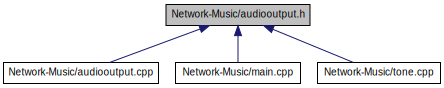
\includegraphics[width=350pt]{audiooutput_8h__dep__incl}
\end{center}
\end{figure}
\subsection*{Classes}
\begin{DoxyCompactItemize}
\item 
class \hyperlink{class_audio_test}{Audio\-Test}
\end{DoxyCompactItemize}

\hypertarget{generator_8cpp}{\section{Network-\/\-Music/generator.cpp File Reference}
\label{generator_8cpp}\index{Network-\/\-Music/generator.\-cpp@{Network-\/\-Music/generator.\-cpp}}
}
{\ttfamily \#include \char`\"{}generator.\-h\char`\"{}}\\*
{\ttfamily \#include $<$qmath.\-h$>$}\\*
{\ttfamily \#include $<$qendian.\-h$>$}\\*
{\ttfamily \#include $<$Q\-Debug$>$}\\*
Include dependency graph for generator.\-cpp\-:\nopagebreak
\begin{figure}[H]
\begin{center}
\leavevmode
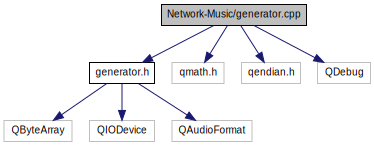
\includegraphics[width=350pt]{generator_8cpp__incl}
\end{center}
\end{figure}

\hypertarget{generator_8h}{\section{Network-\/\-Music/generator.h File Reference}
\label{generator_8h}\index{Network-\/\-Music/generator.\-h@{Network-\/\-Music/generator.\-h}}
}
{\ttfamily \#include $<$Q\-Byte\-Array$>$}\\*
{\ttfamily \#include $<$Q\-I\-O\-Device$>$}\\*
{\ttfamily \#include $<$Q\-Audio\-Format$>$}\\*
Include dependency graph for generator.\-h\-:\nopagebreak
\begin{figure}[H]
\begin{center}
\leavevmode
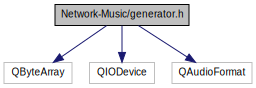
\includegraphics[width=328pt]{generator_8h__incl}
\end{center}
\end{figure}
This graph shows which files directly or indirectly include this file\-:
\nopagebreak
\begin{figure}[H]
\begin{center}
\leavevmode
\includegraphics[width=350pt]{generator_8h__dep__incl}
\end{center}
\end{figure}
\subsection*{Classes}
\begin{DoxyCompactItemize}
\item 
class \hyperlink{class_generator}{Generator}
\end{DoxyCompactItemize}

\hypertarget{main_8cpp}{\section{Network-\/\-Music/main.cpp File Reference}
\label{main_8cpp}\index{Network-\/\-Music/main.\-cpp@{Network-\/\-Music/main.\-cpp}}
}
{\ttfamily \#include $<$Q\-Application$>$}\\*
{\ttfamily \#include $<$Q\-Splash\-Screen$>$}\\*
{\ttfamily \#include $<$Q\-Debug$>$}\\*
{\ttfamily \#include \char`\"{}audiooutput.\-h\char`\"{}}\\*
Include dependency graph for main.\-cpp\-:
\nopagebreak
\begin{figure}[H]
\begin{center}
\leavevmode
\includegraphics[width=350pt]{main_8cpp__incl}
\end{center}
\end{figure}
\subsection*{Functions}
\begin{DoxyCompactItemize}
\item 
int \hyperlink{main_8cpp_a0ddf1224851353fc92bfbff6f499fa97}{main} (int argc, char $\ast$argv\mbox{[}$\,$\mbox{]})
\end{DoxyCompactItemize}


\subsection{Function Documentation}
\hypertarget{main_8cpp_a0ddf1224851353fc92bfbff6f499fa97}{\index{main.\-cpp@{main.\-cpp}!main@{main}}
\index{main@{main}!main.cpp@{main.\-cpp}}
\subsubsection[{main}]{\setlength{\rightskip}{0pt plus 5cm}int main (
\begin{DoxyParamCaption}
\item[{int}]{argc, }
\item[{char $\ast$}]{argv\mbox{[}$\,$\mbox{]}}
\end{DoxyParamCaption}
)}}\label{main_8cpp_a0ddf1224851353fc92bfbff6f499fa97}


Here is the call graph for this function\-:
\nopagebreak
\begin{figure}[H]
\begin{center}
\leavevmode
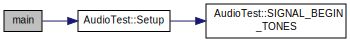
\includegraphics[width=350pt]{main_8cpp_a0ddf1224851353fc92bfbff6f499fa97_cgraph}
\end{center}
\end{figure}



\hypertarget{mainwindow_8cpp}{\section{Network-\/\-Music/mainwindow.cpp File Reference}
\label{mainwindow_8cpp}\index{Network-\/\-Music/mainwindow.\-cpp@{Network-\/\-Music/mainwindow.\-cpp}}
}
{\ttfamily \#include \char`\"{}mainwindow.\-h\char`\"{}}\\*
Include dependency graph for mainwindow.\-cpp\-:\nopagebreak
\begin{figure}[H]
\begin{center}
\leavevmode
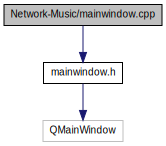
\includegraphics[width=238pt]{mainwindow_8cpp__incl}
\end{center}
\end{figure}

\hypertarget{mainwindow_8h}{\section{Network-\/\-Music/mainwindow.h File Reference}
\label{mainwindow_8h}\index{Network-\/\-Music/mainwindow.\-h@{Network-\/\-Music/mainwindow.\-h}}
}
{\ttfamily \#include $<$Q\-Main\-Window$>$}\\*
Include dependency graph for mainwindow.\-h\-:\nopagebreak
\begin{figure}[H]
\begin{center}
\leavevmode
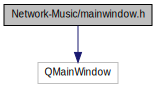
\includegraphics[width=228pt]{mainwindow_8h__incl}
\end{center}
\end{figure}
This graph shows which files directly or indirectly include this file\-:\nopagebreak
\begin{figure}[H]
\begin{center}
\leavevmode
\includegraphics[width=238pt]{mainwindow_8h__dep__incl}
\end{center}
\end{figure}
\subsection*{Classes}
\begin{DoxyCompactItemize}
\item 
class \hyperlink{class_main_window}{Main\-Window}
\end{DoxyCompactItemize}

\hypertarget{packetcapturer_8cpp}{\section{Network-\/\-Music/packetcapturer.cpp File Reference}
\label{packetcapturer_8cpp}\index{Network-\/\-Music/packetcapturer.\-cpp@{Network-\/\-Music/packetcapturer.\-cpp}}
}
{\ttfamily \#include \char`\"{}packetcapturer.\-h\char`\"{}}\\*
{\ttfamily \#include $<$pcap.\-h$>$}\\*
{\ttfamily \#include $<$qdebug.\-h$>$}\\*
{\ttfamily \#include $<$Q\-Application$>$}\\*
Include dependency graph for packetcapturer.\-cpp\-:\nopagebreak
\begin{figure}[H]
\begin{center}
\leavevmode
\includegraphics[width=350pt]{packetcapturer_8cpp__incl}
\end{center}
\end{figure}
\subsection*{Classes}
\begin{DoxyCompactItemize}
\item 
struct \hyperlink{structpacketprocess_1_1sniff__ethernet}{packetprocess\-::sniff\-\_\-ethernet}
\item 
struct \hyperlink{structpacketprocess_1_1sniff__ip}{packetprocess\-::sniff\-\_\-ip}
\item 
struct \hyperlink{structpacketprocess_1_1sniff__tcp}{packetprocess\-::sniff\-\_\-tcp}
\end{DoxyCompactItemize}
\subsection*{Namespaces}
\begin{DoxyCompactItemize}
\item 
namespace \hyperlink{namespacepacketprocess}{packetprocess}
\end{DoxyCompactItemize}
\subsection*{Macros}
\begin{DoxyCompactItemize}
\item 
\#define \hyperlink{packetcapturer_8cpp_ad46b66695494c1720f45142678f354c9}{E\-T\-H\-E\-R\-T\-Y\-P\-E\-\_\-\-E\-A\-P}~(0x888e) /$\ast$ eap authentication $\ast$/
\item 
\#define \hyperlink{packetcapturer_8cpp_aa3b2d149485c29b898ac20524edad389}{T\-Y\-P\-E\-\_\-\-T\-C\-P}~(6)
\item 
\#define \hyperlink{packetcapturer_8cpp_a895709708f8f909cf7b7459491d549e7}{I\-P\-\_\-\-R\-F}~0x8000		/$\ast$ reserved fragment flag $\ast$/
\item 
\#define \hyperlink{packetcapturer_8cpp_ae2473f4a88d141d5298f92a4335b714a}{I\-P\-\_\-\-D\-F}~0x4000		/$\ast$ dont fragment flag $\ast$/
\item 
\#define \hyperlink{packetcapturer_8cpp_ae8afe1e04bb9bad791443556c3b2cd73}{I\-P\-\_\-\-M\-F}~0x2000		/$\ast$ more fragments flag $\ast$/
\item 
\#define \hyperlink{packetcapturer_8cpp_ad059798b16d1f615b5af8770175121ba}{I\-P\-\_\-\-O\-F\-F\-M\-A\-S\-K}~0x1fff	/$\ast$ mask for fragmenting bits $\ast$/
\item 
\#define \hyperlink{packetcapturer_8cpp_a316a88421a4b66af822ec0e097c01f9a}{I\-P\-\_\-\-H\-L}(ip)~(((ip)-\/$>$ip\-\_\-vhl) \& 0x0f)
\item 
\#define \hyperlink{packetcapturer_8cpp_ad79fc88954ed6d1ab77e5fde5e23b864}{I\-P\-\_\-\-V}(ip)~(((ip)-\/$>$ip\-\_\-vhl) $>$$>$ 4)
\item 
\#define \hyperlink{packetcapturer_8cpp_a040e084a163464aace3da0ab5673f97b}{T\-H\-\_\-\-O\-F\-F}(th)~(((th)-\/$>$th\-\_\-offx2 \& 0xf0) $>$$>$ 4)
\item 
\#define \hyperlink{packetcapturer_8cpp_a1cec9b372679734fcd8394d779442ddb}{T\-H\-\_\-\-F\-I\-N}~0x01
\item 
\#define \hyperlink{packetcapturer_8cpp_a91006117f7ae427b957773ab0e80bfa4}{T\-H\-\_\-\-S\-Y\-N}~0x02
\item 
\#define \hyperlink{packetcapturer_8cpp_a7f2ce15991898c8d3397045087c4381f}{T\-H\-\_\-\-R\-S\-T}~0x04
\item 
\#define \hyperlink{packetcapturer_8cpp_a45b9964096064c9a0c84fbddd2c80d38}{T\-H\-\_\-\-P\-U\-S\-H}~0x08
\item 
\#define \hyperlink{packetcapturer_8cpp_a362dae974cf06bab2b79b70f0cde524f}{T\-H\-\_\-\-A\-C\-K}~0x10
\item 
\#define \hyperlink{packetcapturer_8cpp_a7b18ca973f14696013696a00c5235f32}{T\-H\-\_\-\-U\-R\-G}~0x20
\item 
\#define \hyperlink{packetcapturer_8cpp_acb3203940d8aab3eef7dd8ec1e0112db}{T\-H\-\_\-\-E\-C\-E}~0x40
\item 
\#define \hyperlink{packetcapturer_8cpp_a427da5535811ecaae82a11869ea9e1d9}{T\-H\-\_\-\-C\-W\-R}~0x80
\item 
\#define \hyperlink{packetcapturer_8cpp_a618dec9145afa92eb20e74a97625f754}{T\-H\-\_\-\-F\-L\-A\-G\-S}~(\hyperlink{packetcapturer_8cpp_a1cec9b372679734fcd8394d779442ddb}{T\-H\-\_\-\-F\-I\-N}$|$\hyperlink{packetcapturer_8cpp_a91006117f7ae427b957773ab0e80bfa4}{T\-H\-\_\-\-S\-Y\-N}$|$\hyperlink{packetcapturer_8cpp_a7f2ce15991898c8d3397045087c4381f}{T\-H\-\_\-\-R\-S\-T}$|$\hyperlink{packetcapturer_8cpp_a362dae974cf06bab2b79b70f0cde524f}{T\-H\-\_\-\-A\-C\-K}$|$\hyperlink{packetcapturer_8cpp_a7b18ca973f14696013696a00c5235f32}{T\-H\-\_\-\-U\-R\-G}$|$\hyperlink{packetcapturer_8cpp_acb3203940d8aab3eef7dd8ec1e0112db}{T\-H\-\_\-\-E\-C\-E}$|$\hyperlink{packetcapturer_8cpp_a427da5535811ecaae82a11869ea9e1d9}{T\-H\-\_\-\-C\-W\-R})
\end{DoxyCompactItemize}
\subsection*{Typedefs}
\begin{DoxyCompactItemize}
\item 
typedef u\-\_\-int \hyperlink{namespacepacketprocess_a18e81a7f74513cbc9f8881ee72f67abe}{packetprocess\-::tcp\-\_\-seq}
\end{DoxyCompactItemize}
\subsection*{Functions}
\begin{DoxyCompactItemize}
\item 
void \hyperlink{namespacepacketprocess_a17240af943c2d732bb5242e802445a5f}{packetprocess\-::\-Callback\-\_\-\-Process\-Packet} (u\-\_\-char $\ast$useless, const pcap\-\_\-pkthdr $\ast$pkthdr, const u\-\_\-char $\ast$packet)
\end{DoxyCompactItemize}
\subsection*{Variables}
\begin{DoxyCompactItemize}
\item 
u\-\_\-short \hyperlink{namespacepacketprocess_a0ffda1e178a79656e927189b103e8708}{packetprocess\-::recent\-Freq} = 100
\item 
Q\-Object $\ast$ \hyperlink{namespacepacketprocess_ad98eea621960299d54ed1535bf3a605e}{packetprocess\-::parent}
\end{DoxyCompactItemize}


\subsection{Macro Definition Documentation}
\hypertarget{packetcapturer_8cpp_ad46b66695494c1720f45142678f354c9}{\index{packetcapturer.\-cpp@{packetcapturer.\-cpp}!E\-T\-H\-E\-R\-T\-Y\-P\-E\-\_\-\-E\-A\-P@{E\-T\-H\-E\-R\-T\-Y\-P\-E\-\_\-\-E\-A\-P}}
\index{E\-T\-H\-E\-R\-T\-Y\-P\-E\-\_\-\-E\-A\-P@{E\-T\-H\-E\-R\-T\-Y\-P\-E\-\_\-\-E\-A\-P}!packetcapturer.cpp@{packetcapturer.\-cpp}}
\subsubsection[{E\-T\-H\-E\-R\-T\-Y\-P\-E\-\_\-\-E\-A\-P}]{\setlength{\rightskip}{0pt plus 5cm}\#define E\-T\-H\-E\-R\-T\-Y\-P\-E\-\_\-\-E\-A\-P~(0x888e) /$\ast$ eap authentication $\ast$/}}\label{packetcapturer_8cpp_ad46b66695494c1720f45142678f354c9}
\hypertarget{packetcapturer_8cpp_ae2473f4a88d141d5298f92a4335b714a}{\index{packetcapturer.\-cpp@{packetcapturer.\-cpp}!I\-P\-\_\-\-D\-F@{I\-P\-\_\-\-D\-F}}
\index{I\-P\-\_\-\-D\-F@{I\-P\-\_\-\-D\-F}!packetcapturer.cpp@{packetcapturer.\-cpp}}
\subsubsection[{I\-P\-\_\-\-D\-F}]{\setlength{\rightskip}{0pt plus 5cm}\#define I\-P\-\_\-\-D\-F~0x4000		/$\ast$ dont fragment flag $\ast$/}}\label{packetcapturer_8cpp_ae2473f4a88d141d5298f92a4335b714a}
\hypertarget{packetcapturer_8cpp_a316a88421a4b66af822ec0e097c01f9a}{\index{packetcapturer.\-cpp@{packetcapturer.\-cpp}!I\-P\-\_\-\-H\-L@{I\-P\-\_\-\-H\-L}}
\index{I\-P\-\_\-\-H\-L@{I\-P\-\_\-\-H\-L}!packetcapturer.cpp@{packetcapturer.\-cpp}}
\subsubsection[{I\-P\-\_\-\-H\-L}]{\setlength{\rightskip}{0pt plus 5cm}\#define I\-P\-\_\-\-H\-L(
\begin{DoxyParamCaption}
\item[{}]{ip}
\end{DoxyParamCaption}
)~(((ip)-\/$>$ip\-\_\-vhl) \& 0x0f)}}\label{packetcapturer_8cpp_a316a88421a4b66af822ec0e097c01f9a}
\hypertarget{packetcapturer_8cpp_ae8afe1e04bb9bad791443556c3b2cd73}{\index{packetcapturer.\-cpp@{packetcapturer.\-cpp}!I\-P\-\_\-\-M\-F@{I\-P\-\_\-\-M\-F}}
\index{I\-P\-\_\-\-M\-F@{I\-P\-\_\-\-M\-F}!packetcapturer.cpp@{packetcapturer.\-cpp}}
\subsubsection[{I\-P\-\_\-\-M\-F}]{\setlength{\rightskip}{0pt plus 5cm}\#define I\-P\-\_\-\-M\-F~0x2000		/$\ast$ more fragments flag $\ast$/}}\label{packetcapturer_8cpp_ae8afe1e04bb9bad791443556c3b2cd73}
\hypertarget{packetcapturer_8cpp_ad059798b16d1f615b5af8770175121ba}{\index{packetcapturer.\-cpp@{packetcapturer.\-cpp}!I\-P\-\_\-\-O\-F\-F\-M\-A\-S\-K@{I\-P\-\_\-\-O\-F\-F\-M\-A\-S\-K}}
\index{I\-P\-\_\-\-O\-F\-F\-M\-A\-S\-K@{I\-P\-\_\-\-O\-F\-F\-M\-A\-S\-K}!packetcapturer.cpp@{packetcapturer.\-cpp}}
\subsubsection[{I\-P\-\_\-\-O\-F\-F\-M\-A\-S\-K}]{\setlength{\rightskip}{0pt plus 5cm}\#define I\-P\-\_\-\-O\-F\-F\-M\-A\-S\-K~0x1fff	/$\ast$ mask for fragmenting bits $\ast$/}}\label{packetcapturer_8cpp_ad059798b16d1f615b5af8770175121ba}
\hypertarget{packetcapturer_8cpp_a895709708f8f909cf7b7459491d549e7}{\index{packetcapturer.\-cpp@{packetcapturer.\-cpp}!I\-P\-\_\-\-R\-F@{I\-P\-\_\-\-R\-F}}
\index{I\-P\-\_\-\-R\-F@{I\-P\-\_\-\-R\-F}!packetcapturer.cpp@{packetcapturer.\-cpp}}
\subsubsection[{I\-P\-\_\-\-R\-F}]{\setlength{\rightskip}{0pt plus 5cm}\#define I\-P\-\_\-\-R\-F~0x8000		/$\ast$ reserved fragment flag $\ast$/}}\label{packetcapturer_8cpp_a895709708f8f909cf7b7459491d549e7}
\hypertarget{packetcapturer_8cpp_ad79fc88954ed6d1ab77e5fde5e23b864}{\index{packetcapturer.\-cpp@{packetcapturer.\-cpp}!I\-P\-\_\-\-V@{I\-P\-\_\-\-V}}
\index{I\-P\-\_\-\-V@{I\-P\-\_\-\-V}!packetcapturer.cpp@{packetcapturer.\-cpp}}
\subsubsection[{I\-P\-\_\-\-V}]{\setlength{\rightskip}{0pt plus 5cm}\#define I\-P\-\_\-\-V(
\begin{DoxyParamCaption}
\item[{}]{ip}
\end{DoxyParamCaption}
)~(((ip)-\/$>$ip\-\_\-vhl) $>$$>$ 4)}}\label{packetcapturer_8cpp_ad79fc88954ed6d1ab77e5fde5e23b864}
\hypertarget{packetcapturer_8cpp_a362dae974cf06bab2b79b70f0cde524f}{\index{packetcapturer.\-cpp@{packetcapturer.\-cpp}!T\-H\-\_\-\-A\-C\-K@{T\-H\-\_\-\-A\-C\-K}}
\index{T\-H\-\_\-\-A\-C\-K@{T\-H\-\_\-\-A\-C\-K}!packetcapturer.cpp@{packetcapturer.\-cpp}}
\subsubsection[{T\-H\-\_\-\-A\-C\-K}]{\setlength{\rightskip}{0pt plus 5cm}\#define T\-H\-\_\-\-A\-C\-K~0x10}}\label{packetcapturer_8cpp_a362dae974cf06bab2b79b70f0cde524f}
\hypertarget{packetcapturer_8cpp_a427da5535811ecaae82a11869ea9e1d9}{\index{packetcapturer.\-cpp@{packetcapturer.\-cpp}!T\-H\-\_\-\-C\-W\-R@{T\-H\-\_\-\-C\-W\-R}}
\index{T\-H\-\_\-\-C\-W\-R@{T\-H\-\_\-\-C\-W\-R}!packetcapturer.cpp@{packetcapturer.\-cpp}}
\subsubsection[{T\-H\-\_\-\-C\-W\-R}]{\setlength{\rightskip}{0pt plus 5cm}\#define T\-H\-\_\-\-C\-W\-R~0x80}}\label{packetcapturer_8cpp_a427da5535811ecaae82a11869ea9e1d9}
\hypertarget{packetcapturer_8cpp_acb3203940d8aab3eef7dd8ec1e0112db}{\index{packetcapturer.\-cpp@{packetcapturer.\-cpp}!T\-H\-\_\-\-E\-C\-E@{T\-H\-\_\-\-E\-C\-E}}
\index{T\-H\-\_\-\-E\-C\-E@{T\-H\-\_\-\-E\-C\-E}!packetcapturer.cpp@{packetcapturer.\-cpp}}
\subsubsection[{T\-H\-\_\-\-E\-C\-E}]{\setlength{\rightskip}{0pt plus 5cm}\#define T\-H\-\_\-\-E\-C\-E~0x40}}\label{packetcapturer_8cpp_acb3203940d8aab3eef7dd8ec1e0112db}
\hypertarget{packetcapturer_8cpp_a1cec9b372679734fcd8394d779442ddb}{\index{packetcapturer.\-cpp@{packetcapturer.\-cpp}!T\-H\-\_\-\-F\-I\-N@{T\-H\-\_\-\-F\-I\-N}}
\index{T\-H\-\_\-\-F\-I\-N@{T\-H\-\_\-\-F\-I\-N}!packetcapturer.cpp@{packetcapturer.\-cpp}}
\subsubsection[{T\-H\-\_\-\-F\-I\-N}]{\setlength{\rightskip}{0pt plus 5cm}\#define T\-H\-\_\-\-F\-I\-N~0x01}}\label{packetcapturer_8cpp_a1cec9b372679734fcd8394d779442ddb}
\hypertarget{packetcapturer_8cpp_a618dec9145afa92eb20e74a97625f754}{\index{packetcapturer.\-cpp@{packetcapturer.\-cpp}!T\-H\-\_\-\-F\-L\-A\-G\-S@{T\-H\-\_\-\-F\-L\-A\-G\-S}}
\index{T\-H\-\_\-\-F\-L\-A\-G\-S@{T\-H\-\_\-\-F\-L\-A\-G\-S}!packetcapturer.cpp@{packetcapturer.\-cpp}}
\subsubsection[{T\-H\-\_\-\-F\-L\-A\-G\-S}]{\setlength{\rightskip}{0pt plus 5cm}\#define T\-H\-\_\-\-F\-L\-A\-G\-S~({\bf T\-H\-\_\-\-F\-I\-N}$|${\bf T\-H\-\_\-\-S\-Y\-N}$|${\bf T\-H\-\_\-\-R\-S\-T}$|${\bf T\-H\-\_\-\-A\-C\-K}$|${\bf T\-H\-\_\-\-U\-R\-G}$|${\bf T\-H\-\_\-\-E\-C\-E}$|${\bf T\-H\-\_\-\-C\-W\-R})}}\label{packetcapturer_8cpp_a618dec9145afa92eb20e74a97625f754}
\hypertarget{packetcapturer_8cpp_a040e084a163464aace3da0ab5673f97b}{\index{packetcapturer.\-cpp@{packetcapturer.\-cpp}!T\-H\-\_\-\-O\-F\-F@{T\-H\-\_\-\-O\-F\-F}}
\index{T\-H\-\_\-\-O\-F\-F@{T\-H\-\_\-\-O\-F\-F}!packetcapturer.cpp@{packetcapturer.\-cpp}}
\subsubsection[{T\-H\-\_\-\-O\-F\-F}]{\setlength{\rightskip}{0pt plus 5cm}\#define T\-H\-\_\-\-O\-F\-F(
\begin{DoxyParamCaption}
\item[{}]{th}
\end{DoxyParamCaption}
)~(((th)-\/$>$th\-\_\-offx2 \& 0xf0) $>$$>$ 4)}}\label{packetcapturer_8cpp_a040e084a163464aace3da0ab5673f97b}
\hypertarget{packetcapturer_8cpp_a45b9964096064c9a0c84fbddd2c80d38}{\index{packetcapturer.\-cpp@{packetcapturer.\-cpp}!T\-H\-\_\-\-P\-U\-S\-H@{T\-H\-\_\-\-P\-U\-S\-H}}
\index{T\-H\-\_\-\-P\-U\-S\-H@{T\-H\-\_\-\-P\-U\-S\-H}!packetcapturer.cpp@{packetcapturer.\-cpp}}
\subsubsection[{T\-H\-\_\-\-P\-U\-S\-H}]{\setlength{\rightskip}{0pt plus 5cm}\#define T\-H\-\_\-\-P\-U\-S\-H~0x08}}\label{packetcapturer_8cpp_a45b9964096064c9a0c84fbddd2c80d38}
\hypertarget{packetcapturer_8cpp_a7f2ce15991898c8d3397045087c4381f}{\index{packetcapturer.\-cpp@{packetcapturer.\-cpp}!T\-H\-\_\-\-R\-S\-T@{T\-H\-\_\-\-R\-S\-T}}
\index{T\-H\-\_\-\-R\-S\-T@{T\-H\-\_\-\-R\-S\-T}!packetcapturer.cpp@{packetcapturer.\-cpp}}
\subsubsection[{T\-H\-\_\-\-R\-S\-T}]{\setlength{\rightskip}{0pt plus 5cm}\#define T\-H\-\_\-\-R\-S\-T~0x04}}\label{packetcapturer_8cpp_a7f2ce15991898c8d3397045087c4381f}
\hypertarget{packetcapturer_8cpp_a91006117f7ae427b957773ab0e80bfa4}{\index{packetcapturer.\-cpp@{packetcapturer.\-cpp}!T\-H\-\_\-\-S\-Y\-N@{T\-H\-\_\-\-S\-Y\-N}}
\index{T\-H\-\_\-\-S\-Y\-N@{T\-H\-\_\-\-S\-Y\-N}!packetcapturer.cpp@{packetcapturer.\-cpp}}
\subsubsection[{T\-H\-\_\-\-S\-Y\-N}]{\setlength{\rightskip}{0pt plus 5cm}\#define T\-H\-\_\-\-S\-Y\-N~0x02}}\label{packetcapturer_8cpp_a91006117f7ae427b957773ab0e80bfa4}
\hypertarget{packetcapturer_8cpp_a7b18ca973f14696013696a00c5235f32}{\index{packetcapturer.\-cpp@{packetcapturer.\-cpp}!T\-H\-\_\-\-U\-R\-G@{T\-H\-\_\-\-U\-R\-G}}
\index{T\-H\-\_\-\-U\-R\-G@{T\-H\-\_\-\-U\-R\-G}!packetcapturer.cpp@{packetcapturer.\-cpp}}
\subsubsection[{T\-H\-\_\-\-U\-R\-G}]{\setlength{\rightskip}{0pt plus 5cm}\#define T\-H\-\_\-\-U\-R\-G~0x20}}\label{packetcapturer_8cpp_a7b18ca973f14696013696a00c5235f32}
\hypertarget{packetcapturer_8cpp_aa3b2d149485c29b898ac20524edad389}{\index{packetcapturer.\-cpp@{packetcapturer.\-cpp}!T\-Y\-P\-E\-\_\-\-T\-C\-P@{T\-Y\-P\-E\-\_\-\-T\-C\-P}}
\index{T\-Y\-P\-E\-\_\-\-T\-C\-P@{T\-Y\-P\-E\-\_\-\-T\-C\-P}!packetcapturer.cpp@{packetcapturer.\-cpp}}
\subsubsection[{T\-Y\-P\-E\-\_\-\-T\-C\-P}]{\setlength{\rightskip}{0pt plus 5cm}\#define T\-Y\-P\-E\-\_\-\-T\-C\-P~(6)}}\label{packetcapturer_8cpp_aa3b2d149485c29b898ac20524edad389}

\hypertarget{packetcapturer_8h}{\section{Network-\/\-Music/packetcapturer.h File Reference}
\label{packetcapturer_8h}\index{Network-\/\-Music/packetcapturer.\-h@{Network-\/\-Music/packetcapturer.\-h}}
}
{\ttfamily \#include $<$Q\-Object$>$}\\*
{\ttfamily \#include $<$pcap.\-h$>$}\\*
{\ttfamily \#include $<$sys/socket.\-h$>$}\\*
{\ttfamily \#include $<$netinet/in.\-h$>$}\\*
{\ttfamily \#include $<$netinet/ip.\-h$>$}\\*
{\ttfamily \#include $<$netinet/ether.\-h$>$}\\*
{\ttfamily \#include $<$net/ethernet.\-h$>$}\\*
{\ttfamily \#include $<$arpa/inet.\-h$>$}\\*
Include dependency graph for packetcapturer.\-h\-:\nopagebreak
\begin{figure}[H]
\begin{center}
\leavevmode
\includegraphics[width=350pt]{packetcapturer_8h__incl}
\end{center}
\end{figure}
This graph shows which files directly or indirectly include this file\-:\nopagebreak
\begin{figure}[H]
\begin{center}
\leavevmode
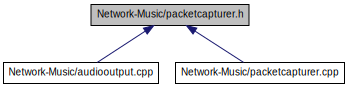
\includegraphics[width=350pt]{packetcapturer_8h__dep__incl}
\end{center}
\end{figure}
\subsection*{Classes}
\begin{DoxyCompactItemize}
\item 
class \hyperlink{class_packet_capturer}{Packet\-Capturer}
\end{DoxyCompactItemize}
\subsection*{Macros}
\begin{DoxyCompactItemize}
\item 
\#define \hyperlink{packetcapturer_8h_a3f5b604fac0a778d4d05140ac486303a}{S\-I\-Z\-E\-\_\-\-E\-T\-H\-E\-R\-N\-E\-T}~14
\end{DoxyCompactItemize}


\subsection{Macro Definition Documentation}
\hypertarget{packetcapturer_8h_a3f5b604fac0a778d4d05140ac486303a}{\index{packetcapturer.\-h@{packetcapturer.\-h}!S\-I\-Z\-E\-\_\-\-E\-T\-H\-E\-R\-N\-E\-T@{S\-I\-Z\-E\-\_\-\-E\-T\-H\-E\-R\-N\-E\-T}}
\index{S\-I\-Z\-E\-\_\-\-E\-T\-H\-E\-R\-N\-E\-T@{S\-I\-Z\-E\-\_\-\-E\-T\-H\-E\-R\-N\-E\-T}!packetcapturer.h@{packetcapturer.\-h}}
\subsubsection[{S\-I\-Z\-E\-\_\-\-E\-T\-H\-E\-R\-N\-E\-T}]{\setlength{\rightskip}{0pt plus 5cm}\#define S\-I\-Z\-E\-\_\-\-E\-T\-H\-E\-R\-N\-E\-T~14}}\label{packetcapturer_8h_a3f5b604fac0a778d4d05140ac486303a}

\hypertarget{_r_e_a_d_m_e_8md}{\section{Network-\/\-Music/\-R\-E\-A\-D\-M\-E.md File Reference}
\label{_r_e_a_d_m_e_8md}\index{Network-\/\-Music/\-R\-E\-A\-D\-M\-E.\-md@{Network-\/\-Music/\-R\-E\-A\-D\-M\-E.\-md}}
}

\hypertarget{tone_8cpp}{\section{Network-\/\-Music/tone.cpp File Reference}
\label{tone_8cpp}\index{Network-\/\-Music/tone.\-cpp@{Network-\/\-Music/tone.\-cpp}}
}
{\ttfamily \#include \char`\"{}tone.\-h\char`\"{}}\\*
{\ttfamily \#include \char`\"{}audiooutput.\-h\char`\"{}}\\*
{\ttfamily \#include $<$Q\-Debug$>$}\\*
{\ttfamily \#include $<$Q\-Thread$>$}\\*
Include dependency graph for tone.\-cpp\-:
\nopagebreak
\begin{figure}[H]
\begin{center}
\leavevmode
\includegraphics[width=350pt]{tone_8cpp__incl}
\end{center}
\end{figure}
\subsection*{Variables}
\begin{DoxyCompactItemize}
\item 
const int \hyperlink{tone_8cpp_aa02e50dd3f5e12d36ce6a7255c2c459b}{Duration\-Seconds} = 1
\end{DoxyCompactItemize}


\subsection{Variable Documentation}
\hypertarget{tone_8cpp_aa02e50dd3f5e12d36ce6a7255c2c459b}{\index{tone.\-cpp@{tone.\-cpp}!Duration\-Seconds@{Duration\-Seconds}}
\index{Duration\-Seconds@{Duration\-Seconds}!tone.cpp@{tone.\-cpp}}
\subsubsection[{Duration\-Seconds}]{\setlength{\rightskip}{0pt plus 5cm}const int Duration\-Seconds = 1}}\label{tone_8cpp_aa02e50dd3f5e12d36ce6a7255c2c459b}

\hypertarget{tone_8h}{\section{Network-\/\-Music/tone.h File Reference}
\label{tone_8h}\index{Network-\/\-Music/tone.\-h@{Network-\/\-Music/tone.\-h}}
}
{\ttfamily \#include $<$Q\-Audio\-Device\-Info$>$}\\*
{\ttfamily \#include $<$Q\-Audio\-Output$>$}\\*
{\ttfamily \#include \char`\"{}generator.\-h\char`\"{}}\\*
Include dependency graph for tone.\-h\-:\nopagebreak
\begin{figure}[H]
\begin{center}
\leavevmode
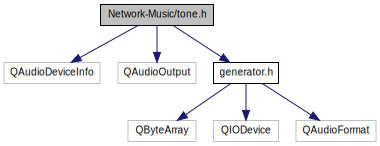
\includegraphics[width=350pt]{tone_8h__incl}
\end{center}
\end{figure}
This graph shows which files directly or indirectly include this file\-:
\nopagebreak
\begin{figure}[H]
\begin{center}
\leavevmode
\includegraphics[width=350pt]{tone_8h__dep__incl}
\end{center}
\end{figure}
\subsection*{Classes}
\begin{DoxyCompactItemize}
\item 
class \hyperlink{classtone}{tone}
\end{DoxyCompactItemize}

\hypertarget{tonemanager_8cpp}{\section{Network-\/\-Music/tonemanager.cpp File Reference}
\label{tonemanager_8cpp}\index{Network-\/\-Music/tonemanager.\-cpp@{Network-\/\-Music/tonemanager.\-cpp}}
}
{\ttfamily \#include \char`\"{}tonemanager.\-h\char`\"{}}\\*
{\ttfamily \#include \char`\"{}generator.\-h\char`\"{}}\\*
{\ttfamily \#include \char`\"{}tone.\-h\char`\"{}}\\*
{\ttfamily \#include $<$Q\-Debug$>$}\\*
{\ttfamily \#include $<$Q\-Thread$>$}\\*
Include dependency graph for tonemanager.\-cpp\-:
\nopagebreak
\begin{figure}[H]
\begin{center}
\leavevmode
\includegraphics[width=350pt]{tonemanager_8cpp__incl}
\end{center}
\end{figure}
\subsection*{Macros}
\begin{DoxyCompactItemize}
\item 
\#define \hyperlink{tonemanager_8cpp_a5e6855de8203fe9ae34cf63f68799e98}{T\-O\-N\-E\-\_\-\-C\-O\-U\-N\-T}~(5)
\end{DoxyCompactItemize}


\subsection{Macro Definition Documentation}
\hypertarget{tonemanager_8cpp_a5e6855de8203fe9ae34cf63f68799e98}{\index{tonemanager.\-cpp@{tonemanager.\-cpp}!T\-O\-N\-E\-\_\-\-C\-O\-U\-N\-T@{T\-O\-N\-E\-\_\-\-C\-O\-U\-N\-T}}
\index{T\-O\-N\-E\-\_\-\-C\-O\-U\-N\-T@{T\-O\-N\-E\-\_\-\-C\-O\-U\-N\-T}!tonemanager.cpp@{tonemanager.\-cpp}}
\subsubsection[{T\-O\-N\-E\-\_\-\-C\-O\-U\-N\-T}]{\setlength{\rightskip}{0pt plus 5cm}\#define T\-O\-N\-E\-\_\-\-C\-O\-U\-N\-T~(5)}}\label{tonemanager_8cpp_a5e6855de8203fe9ae34cf63f68799e98}

\hypertarget{tonemanager_8h}{\section{Network-\/\-Music/tonemanager.h File Reference}
\label{tonemanager_8h}\index{Network-\/\-Music/tonemanager.\-h@{Network-\/\-Music/tonemanager.\-h}}
}
{\ttfamily \#include $<$Q\-Object$>$}\\*
{\ttfamily \#include $<$Q\-Hash$>$}\\*
{\ttfamily \#include $<$Q\-List$>$}\\*
{\ttfamily \#include $<$Q\-Audio\-Format$>$}\\*
Include dependency graph for tonemanager.\-h\-:
\nopagebreak
\begin{figure}[H]
\begin{center}
\leavevmode
\includegraphics[width=350pt]{tonemanager_8h__incl}
\end{center}
\end{figure}
This graph shows which files directly or indirectly include this file\-:
\nopagebreak
\begin{figure}[H]
\begin{center}
\leavevmode
\includegraphics[width=350pt]{tonemanager_8h__dep__incl}
\end{center}
\end{figure}
\subsection*{Classes}
\begin{DoxyCompactItemize}
\item 
struct \hyperlink{struct_tone_object}{Tone\-Object}
\item 
class \hyperlink{class_tone_manager}{Tone\-Manager}
\end{DoxyCompactItemize}

\printindex
\end{document}
